\section{Smith's decomposition}\label{sec:smith}

Smith's decomposition of $K_q=P(-2,3,q)$ is \eqref{eq:family} with the earring on the $-2$ band,
$T_1=\Qh{-1/2}$ and $T_2=Q_{1/3}+Q_{1/q}$ \cite{Smith}.  The red
curve $\Rnat(\Qh{-1/2})$ does not depend on $q$; the blue curve is Smith's holonomy-perturbed curve
$\Rp_t(Q_{1/3}+Q_{1/q})$.  In contrast with the decomposition of Section~\ref{sec:sheared}, the
pairing of these two curves with zero bounding cochain does not have the rank of $\Inat(K_q)$: at $q=7$
it is $7$ rather than $9$ (Proposition~\ref{prop:q7-typeD}), and the finite statistics of
\S\ref{sec:compute} differ from $q+2$ by $\pm2$ for $q=5,7,11,13$.  Conditional on the conjecture of
Cazassus, Herald, Kirk and Kotelskiy \cite[Conj.~D]{CHKK}, Smith deduces that $T_2$ must carry a
nonzero bounding cochain when $q=5$ \cite[proof of Thm.~5.9]{Smith}.  At $q=7$ we work in the two-arc
algebra of Section~\ref{sec:background}: local smoothings of the blue curve give Maurer--Cartan
elements to all orders, and a second closure selects one homotopy class among them, conditionally on a
localization hypothesis.  Section~\ref{sec:khovanov} relates the selected class to the Khovanov
invariant of $T_2$.  Statements labelled \emph{Computation} are outputs of the finite procedures of
\S\ref{sec:compute} and are recorded as data; the statement labelled \emph{Hypothesis} is assumed,
not proved.

\subsection{Piecewise-linear models and Smith's cross-resolution}\label{ss:models}
We work in Smith's coordinates \eqref{eq:smith-coords}, with the corner rule for rational lines and
the fiber-product description of Conway sums recalled in \S\ref{ss:smith-chart}.  As Smith does, we
call the images of the lines $\gamma=0$ and $\gamma=\pi$ the \emph{edges} of the pillowcase, and the
circles of representations that a Conway sum acquires over them \emph{edge circles}
\cite[Thms.~3.15 and 3.26]{Smith}.  Smith's perturbation resolves each internal edge circle by a
diagonal cut-and-paste \cite[Thm.~4.22]{Smith}, which replaces it by two arcs crossing once; we call
these arcs \emph{connectors}, and the remaining arcs of the resolved curve, which come from the fiber
product, \emph{inherited strands}.  The earring curve $E_r$ of $\Qh{r}$ is a Herald--Kirk
figure-eight, the doubled arc closing through the corner folds with one pinch \cite[Def.~6.7]{HK}; this
specifies a finite curve, not a bounding cochain.  The closing tangle enters the pairing through its
mirror image, so $E_r$ surrounds the line of $Q_{-r}$ (\S\ref{ss:kh-smith}); for instance the red
curve $E_{-1/2}=\Rnat(\Qh{-1/2})$ lies along the line of slope $1/2$.

Write $L_{q,\mathrm{PL}}$ for the piecewise-linear curve obtained from the lines of slopes $1/3$ and
$1/q$ through $(0,0)$ by the fiber product and the crossed local pairing at every edge circle.  These
lines are the translates by $(0,\pi)$ of the lines of $Q_{1/3}$ and $Q_{1/q}$, and since the fiber
product adds the $\theta$-coordinates the two shifts cancel: both fiber products have the same image
and the same edge circles.  The model represents Smith's perturbed curve for negative values of his
perturbation parameter (Remark~\ref{rem:sign}).  The red curve $\Rnat(\Qh{-1/2})$ is one immersed
circle with one pinch; the blue curve has $q-1$ resolved edge circles and is a single proper immersed
arc.  The model $L_{q,\mathrm{PL}}$ has $40$, $82$ and $240$ transverse self-intersections at
$q=5,7,11$.  These are counts for the model: the number is not invariant under regular homotopy, and a
numerical trace of Smith's perturbed curve at $q=7$ has $50$ (Remark~\ref{rem:analytic}).  At $q=7$
the model also has twelve tangential self-contacts on the edges, where connectors meet inherited
strands without crossing; we remove them by a small perturbation that creates no crossings.  We
require $\gcd(q,3)=1$, since otherwise corner circles appear; this excludes $q=3,9,15,\dots$ from the
members computed here, but not from Theorem~\ref{thm:inat}.

\begin{proposition}[Smith's cross-resolution and the model]\label{prop:smith-main}
Let $q$ be odd and $\gcd(q,3)=1$.
\begin{enumerate}
\item[(a)] The fiber product of the rational lines of slopes $1/3$ and $1/q$ has $q-1$ edge circles,
all internal, and no corner circles.
\item[(b)] For all sufficiently small nonzero values $t$ of Smith's $C_3$-perturbation parameter,
after an arbitrarily small additional perturbation where Smith's construction requires one,
$\Rp_t(Q_{1/3}+Q_{1/q})$ contains a subspace homeomorphic to the curve obtained from the fiber
product by replacing each internal circle with two intervals joined to its ends crosswise; this is
the pairing used to define $L_{q,\mathrm{PL}}$.  As $t\to0$ the image of each new interval approaches
the image of the corresponding circle.  The remaining components are circles, the \emph{auxiliary
components}.
\item[(c)] For a fixed complementary tangle, there is an arbitrarily small perturbation of it for
which the Floer pairing with $\Rp_t(Q_{1/3}+Q_{1/q})$ equals the pairing with its main components.
This remains valid when either tangle carries an earring.
\end{enumerate}
\end{proposition}

\begin{proof}
Smith identifies the two rational character varieties with straight intervals of slopes $1/3$ and
$1/q$ \cite[Prop.~2.27]{Smith}, and rational tangles of finite slope form a good pair without
preliminary perturbations \cite[example following Thm.~3.26]{Smith}.  Because the denominators $3$ and
$q$ are coprime, the sum has no corner circles \cite[discussion following Prop.~5.8]{Smith}, so every
edge circle is internal.  This is (a).  For $t>0$, part (b) is Smith's cross-resolution theorem
\cite[Thm.~4.22]{Smith}, together with his remark preceding \cite[Thm.~4.20]{Smith} that an
arbitrarily small additional perturbation makes the relevant spaces manifolds when transversality
fails.  For $t<0$ it follows from the case of $-t$: the homeomorphism $\hat\sm$ of
Remark~\ref{rem:sign} maps $\Rp_{-t}(Q_{1/3}+Q_{1/q})$ onto $\Rp_t(Q_{1/3}+Q_{1/q})$ and the
unperturbed fiber product onto itself, and it acts on the pillowcase of the sum by the translation
$(\gamma,\theta)\mapsto(\gamma+\pi,\theta)$.  Part (c) is Smith's auxiliary-component result
\cite[Prop.~5.7]{Smith}, which includes the earring case; its proof uses only that the auxiliary
components converge to finitely many points of $\Pst$ as $t\to0$, and by the same homeomorphism this
also holds for $t<0$.
\end{proof}

Smith states informally that \cite[Thm.~4.22]{Smith} determines the image of the main component up
to regular homotopy (\cite[caption of Fig.~3]{Smith} and the outline of the proof in his
introduction); the formal statement gives the homeomorphism type and the convergence in (b).  We use
$L_{q,\mathrm{PL}}$ as a representative of that regular-homotopy class, but no proof below depends on
this identification; at $q=7$ the type-D encoding of a traced copy of Smith's curve is strictly
isomorphic to that of $L_{7,\mathrm{PL}}$ (Remark~\ref{rem:analytic}).

\begin{remark}[The sign of the perturbation]\label{rem:sign}
In Smith's configuration $C_3$ the summands are glued along two inner boundary spheres, with
pillowcases $P_1$ and $P_2$, and the sum is read off on the outer sphere, with pillowcase $P_3$; write
$C_{3,t}$ for the perturbed character variety of the configuration.  Its representations are
parametrized by the images of the meridians $a,b,c$ of the outer sphere and of a meridian $x$ of the
first inner sphere: the perturbation element is $p=\exp\bigl(t\operatorname{Im}(ac^{-1}x)\bigr)$, the
remaining meridians are $d=ca^{-1}b$ and $y=xp^{-1}a^{-1}pb$, and the perturbed variety is cut out by
$\operatorname{Re}(y)=0$ \cite[Prop.~4.1 and (4.1.1)]{Smith}.  The substitution
$\sm\colon(x,t)\mapsto(-x,-t)$ leaves $p$ and $d$ unchanged and replaces $y$ by $-y$, so it maps the
perturbed variety for $t$ onto that for $-t$.  It is the identity on $P_3$, and a direct computation
with Smith's boundary words \cite[Fig.~20]{Smith} shows that it acts on $P_1$ and on $P_2$ by the
translation $(\gamma,\theta)\mapsto(\gamma,\theta+\pi)$.  For odd $q$ a line of slope $1/q$ is
invariant under translation by $(\pi,\pi)$, so translation by $(0,\pi)$ carries the line of slope
$1/q$ through $(0,0)$ to the line through $(\pi,0)$ and $(0,\pi)$.  Consequently $\sm$ carries the
composition of $C_{3,t}$ with the lines of slopes $1/3$ and $1/q$ through $(0,0)$, for $t>0$, onto the
composition of $C_{3,-t}$ with the lines of $Q_{1/3}$ and $Q_{1/q}$, without moving the image in $P_3$.
Hence the piecewise-linear model, which is built from the lines through $(0,0)$ and compared with
their composition for $t>0$, represents the main component of $\Rp_t(Q_{1/3}+Q_{1/q})$ in Smith's
coordinates for small $t<0$, which is the convention of \S\ref{ss:smith-chart}.

The substitution $b\mapsto-b$ is also a symmetry of Smith's equations for each $t$, since $p$ does not
involve $b$ and $y$ changes sign; it translates each of $P_1,P_2,P_3$ by
$(\gamma,\theta)\mapsto(\gamma+\pi,\theta)$.  The composite $\hat\sm\colon(b,x,t)\mapsto(-b,-x,-t)$
therefore translates $P_1$ and $P_2$ by $(\pi,\pi)$, which preserves the lines of $Q_{1/3}$ and
$Q_{1/q}$, and $P_3$ by $(\pi,0)$, so the curve for $t>0$ is the translate by $(\pi,0)$ of the curve
for $-t$.  This translation is a symplectomorphism of $\Pst$ that permutes the corners, but the
translated curve is a different representative, and pairings of its smoothings with the earrings can
differ from those for $t<0$ (Remark~\ref{rem:sign-pairings}).
\end{remark}

\begin{figure}[ht]
\centering
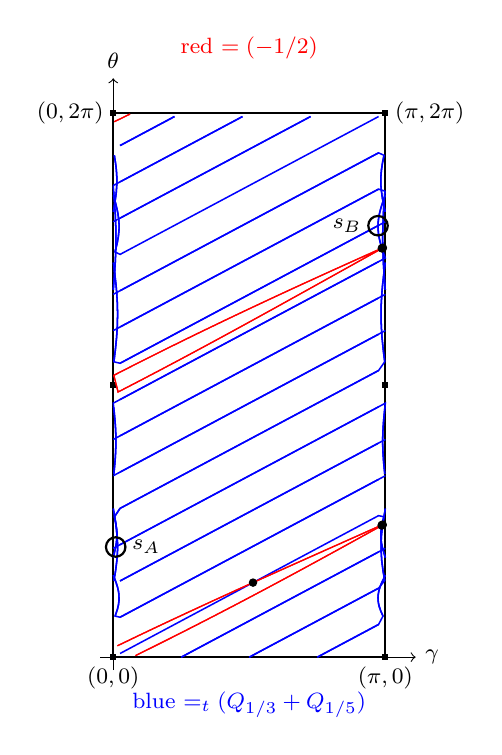
\begin{tikzpicture}[scale=1.1]
% Figure curves generated by pillowcase/make_figure.py (inlined)
% AUTO-GENERATED by pillowcase/make_figure.py -- the q=5 PL model curves.
%% blue folded into 52 pieces; red (both lifts) into 10 pieces.
\draw[thick] (0,0) rectangle (3.14159,6.28319);
\foreach \y in {0,3.14159,6.28319}{\fill (-0.035,\y-0.035) rectangle (0.035,\y+0.035); \fill (3.14159-0.035,\y-0.035) rectangle (3.14159+0.035,\y+0.035);}
\node[below] at (0,0) {\footnotesize $(0,0)$};
\node[below] at (3.1416,0) {\footnotesize $(\pi,0)$};
\node[left] at (0,6.2832) {\footnotesize $(0,2\pi)$};
\node[right] at (3.1416,6.2832) {\footnotesize $(\pi,2\pi)$};
\draw[->] (-0.15,0)--(3.4916,0) node[right] {\footnotesize $\gamma$};
\draw[->] (0,-0.15)--(0,6.6832) node[above] {\footnotesize $\theta$};
\draw[blue,line width=0.55pt] (0.0000,5.4454) -- (0.1571,5.5292) -- (0.3142,5.6130) -- (0.4712,5.6968) -- (0.6283,5.7805) -- (0.7854,5.8643) -- (0.9425,5.9481) -- (1.0996,6.0319) -- (1.2566,6.1156) -- (1.4137,6.1994) -- (1.4923,6.2413);
\draw[blue,line width=0.55pt] (1.5708,0.0000) -- (1.7279,0.0838) -- (1.8850,0.1676) -- (2.0420,0.2513) -- (2.1991,0.3351) -- (2.3562,0.4189) -- (2.5133,0.5027) -- (2.6704,0.5864) -- (2.8274,0.6702) -- (2.9845,0.7540) -- (3.0631,0.7959);
\draw[blue,line width=0.55pt] (3.1336,0.8836) -- (3.1150,0.9948) -- (3.1000,1.1126) -- (3.0923,1.2305) -- (3.0926,1.3352) -- (3.0974,1.4137) -- (3.1056,1.4923) -- (3.1186,1.5839) -- (3.1411,1.7148);
\draw[blue,line width=0.55pt] (3.1402,4.5553) -- (3.1221,4.4113) -- (3.1092,4.2935) -- (3.1012,4.2019) -- (3.0937,4.0710) -- (3.0916,3.9532) -- (3.0947,3.8223) -- (3.1030,3.6914) -- (3.1173,3.5474) -- (3.1341,3.4099) -- (3.0631,3.3091) -- (2.9060,3.2254) -- (2.7489,3.1416) -- (2.5918,3.0578) -- (2.4347,2.9740) -- (2.2777,2.8903) -- (2.1206,2.8065) -- (1.9635,2.7227) -- (1.8064,2.6389) -- (1.6493,2.5552) -- (1.4923,2.4714) -- (1.3352,2.3876) -- (1.1781,2.3038) -- (1.0210,2.2201) -- (0.8639,2.1363) -- (0.7069,2.0525) -- (0.5498,1.9687) -- (0.3927,1.8850) -- (0.2356,1.8012) -- (0.0785,1.7174) -- (0.0135,1.6205) -- (0.0299,1.5420) -- (0.0392,1.4713) -- (0.0418,1.4085) -- (0.0394,1.3535) -- (0.0339,1.3064) -- (0.0258,1.2593) -- (0.0004,1.1493);
\draw[blue,line width=0.55pt] (0.0011,5.1417) -- (0.0163,5.2281) -- (0.0338,5.3538) -- (0.0411,5.4559) -- (0.0412,5.5423) -- (0.0363,5.6208) -- (0.0273,5.6994) -- (0.0126,5.7936);
\draw[blue,line width=0.55pt] (0.0785,5.9062) -- (0.2356,5.9900) -- (0.3927,6.0737) -- (0.5498,6.1575) -- (0.7069,6.2413);
\draw[blue,line width=0.55pt] (0.7854,0.0000) -- (0.9425,0.0838) -- (1.0996,0.1676) -- (1.2566,0.2513) -- (1.4137,0.3351) -- (1.5708,0.4189) -- (1.7279,0.5027) -- (1.8850,0.5864) -- (2.0420,0.6702) -- (2.1991,0.7540) -- (2.3562,0.8378) -- (2.5133,0.9215) -- (2.6704,1.0053) -- (2.8274,1.0891) -- (2.9845,1.1729) -- (3.0631,1.2147);
\draw[blue,line width=0.55pt] (3.1416,5.0265) -- (2.9845,4.9428) -- (2.8274,4.8590) -- (2.6704,4.7752) -- (2.5133,4.6914) -- (2.3562,4.6077) -- (2.1991,4.5239) -- (2.0420,4.4401) -- (1.8850,4.3563) -- (1.7279,4.2726) -- (1.5708,4.1888) -- (1.4137,4.1050) -- (1.2566,4.0212) -- (1.0996,3.9375) -- (0.9425,3.8537) -- (0.7854,3.7699) -- (0.6283,3.6861) -- (0.4712,3.6024) -- (0.3142,3.5186) -- (0.1571,3.4348) -- (0.0785,3.3929);
\draw[blue,line width=0.55pt] (0.0075,3.4099) -- (0.0243,3.5474) -- (0.0385,3.6914) -- (0.0469,3.8223) -- (0.0500,3.9532) -- (0.0479,4.0710) -- (0.0404,4.2019) -- (0.0324,4.2935) -- (0.0194,4.4113) -- (0.0014,4.5553);
\draw[blue,line width=0.55pt] (0.0005,1.7148) -- (0.0229,1.5839) -- (0.0360,1.4923) -- (0.0442,1.4137) -- (0.0489,1.3352) -- (0.0493,1.2305) -- (0.0416,1.1126) -- (0.0266,0.9948) -- (0.0080,0.8836);
\draw[blue,line width=0.55pt] (0.0785,0.8796) -- (0.2356,0.9634) -- (0.3927,1.0472) -- (0.5498,1.1310) -- (0.7069,1.2147) -- (0.8639,1.2985) -- (1.0210,1.3823) -- (1.1781,1.4661) -- (1.3352,1.5499) -- (1.4923,1.6336) -- (1.6493,1.7174) -- (1.8064,1.8012) -- (1.9635,1.8850) -- (2.1206,1.9687) -- (2.2777,2.0525) -- (2.4347,2.1363) -- (2.5918,2.2201) -- (2.7489,2.3038) -- (2.9060,2.3876) -- (3.0631,2.4714);
\draw[blue,line width=0.55pt] (3.1416,3.7699) -- (2.9845,3.6861) -- (2.8274,3.6024) -- (2.6704,3.5186) -- (2.5133,3.4348) -- (2.3562,3.3510) -- (2.1991,3.2673) -- (2.0420,3.1835) -- (1.8850,3.0997) -- (1.7279,3.0159) -- (1.5708,2.9322) -- (1.4137,2.8484) -- (1.2566,2.7646) -- (1.0996,2.6808) -- (0.9425,2.5970) -- (0.7854,2.5133) -- (0.6283,2.4295) -- (0.4712,2.3457) -- (0.3142,2.2619) -- (0.1571,2.1782) -- (0.0785,2.1363);
\draw[blue,line width=0.55pt] (0.0000,4.1888) -- (0.1571,4.2726) -- (0.3142,4.3563) -- (0.4712,4.4401) -- (0.6283,4.5239) -- (0.7854,4.6077) -- (0.9425,4.6914) -- (1.0996,4.7752) -- (1.2566,4.8590) -- (1.4137,4.9428) -- (1.5708,5.0265) -- (1.7279,5.1103) -- (1.8850,5.1941) -- (2.0420,5.2779) -- (2.1991,5.3617) -- (2.3562,5.4454) -- (2.5133,5.5292) -- (2.6704,5.6130) -- (2.8274,5.6968) -- (2.9845,5.7805) -- (3.0631,5.8224);
\draw[blue,line width=0.55pt] (3.1258,5.7936) -- (3.1072,5.6994) -- (3.0959,5.6208) -- (3.0898,5.5423) -- (3.0898,5.4559) -- (3.0936,5.4009) -- (3.1075,5.2988) -- (3.1211,5.2281) -- (3.1402,5.1417);
\draw[blue,line width=0.55pt] (3.1411,1.1493) -- (3.1174,1.2278) -- (3.1036,1.2828) -- (3.0950,1.3299) -- (3.0900,1.3771) -- (3.0896,1.4399) -- (3.0941,1.4870) -- (3.1040,1.5420) -- (3.1247,1.6205) -- (3.0631,1.6336) -- (2.9060,1.5499) -- (2.7489,1.4661) -- (2.5918,1.3823) -- (2.4347,1.2985) -- (2.2777,1.2147) -- (2.1206,1.1310) -- (1.9635,1.0472) -- (1.8064,0.9634) -- (1.6493,0.8796) -- (1.4923,0.7959) -- (1.3352,0.7121) -- (1.1781,0.6283) -- (1.0210,0.5445) -- (0.8639,0.4608) -- (0.7069,0.3770) -- (0.5498,0.2932) -- (0.3927,0.2094) -- (0.2356,0.1257) -- (0.0785,0.0419) -- (0.0785,0.0419) -- (0.2356,0.1257) -- (0.3927,0.2094) -- (0.5498,0.2932) -- (0.7069,0.3770) -- (0.8639,0.4608) -- (1.0210,0.5445) -- (1.1781,0.6283) -- (1.3352,0.7121) -- (1.4923,0.7959) -- (1.6493,0.8796) -- (1.8064,0.9634) -- (1.9635,1.0472) -- (2.1206,1.1310) -- (2.2777,1.2147) -- (2.4347,1.2985) -- (2.5918,1.3823) -- (2.7489,1.4661) -- (2.9060,1.5499) -- (3.0631,1.6336);
\draw[blue,line width=0.55pt] (3.1247,1.6205) -- (3.1040,1.5420) -- (3.0941,1.4870) -- (3.0896,1.4399) -- (3.0900,1.3771) -- (3.0950,1.3299) -- (3.1036,1.2828) -- (3.1174,1.2278) -- (3.1411,1.1493);
\draw[blue,line width=0.55pt] (3.1402,5.1417) -- (3.1211,5.2281) -- (3.1075,5.2988) -- (3.0936,5.4009) -- (3.0898,5.4559) -- (3.0898,5.5423) -- (3.0959,5.6208) -- (3.1072,5.6994) -- (3.1258,5.7936) -- (3.0631,5.8224) -- (2.9060,5.7386) -- (2.7489,5.6549) -- (2.5918,5.5711) -- (2.4347,5.4873) -- (2.2777,5.4035) -- (2.1206,5.3198) -- (1.9635,5.2360) -- (1.8064,5.1522) -- (1.6493,5.0684) -- (1.4923,4.9847) -- (1.3352,4.9009) -- (1.1781,4.8171) -- (1.0210,4.7333) -- (0.8639,4.6496) -- (0.7069,4.5658) -- (0.5498,4.4820) -- (0.3927,4.3982) -- (0.2356,4.3145) -- (0.0785,4.2307);
\draw[blue,line width=0.55pt] (0.0000,2.0944) -- (0.1571,2.1782) -- (0.3142,2.2619) -- (0.4712,2.3457) -- (0.6283,2.4295) -- (0.7854,2.5133) -- (0.9425,2.5970) -- (1.0996,2.6808) -- (1.2566,2.7646) -- (1.4137,2.8484) -- (1.5708,2.9322) -- (1.7279,3.0159) -- (1.8850,3.0997) -- (2.0420,3.1835) -- (2.1991,3.2673) -- (2.3562,3.3510) -- (2.5133,3.4348) -- (2.6704,3.5186) -- (2.8274,3.6024) -- (2.9845,3.6861) -- (3.0631,3.7280);
\draw[blue,line width=0.55pt] (3.1416,2.5133) -- (2.9845,2.4295) -- (2.8274,2.3457) -- (2.6704,2.2619) -- (2.5133,2.1782) -- (2.3562,2.0944) -- (2.1991,2.0106) -- (2.0420,1.9268) -- (1.8850,1.8431) -- (1.7279,1.7593) -- (1.5708,1.6755) -- (1.4137,1.5917) -- (1.2566,1.5080) -- (1.0996,1.4242) -- (0.9425,1.3404) -- (0.7854,1.2566) -- (0.6283,1.1729) -- (0.4712,1.0891) -- (0.3142,1.0053) -- (0.1571,0.9215) -- (0.0785,0.8796);
\draw[blue,line width=0.55pt] (0.0080,0.8836) -- (0.0266,0.9948) -- (0.0416,1.1126) -- (0.0493,1.2305) -- (0.0489,1.3352) -- (0.0442,1.4137) -- (0.0360,1.4923) -- (0.0229,1.5839) -- (0.0005,1.7148);
\draw[blue,line width=0.55pt] (0.0014,4.5553) -- (0.0194,4.4113) -- (0.0324,4.2935) -- (0.0404,4.2019) -- (0.0479,4.0710) -- (0.0500,3.9532) -- (0.0469,3.8223) -- (0.0385,3.6914) -- (0.0243,3.5474) -- (0.0075,3.4099) -- (0.0785,3.3929) -- (0.2356,3.4767) -- (0.3927,3.5605) -- (0.5498,3.6442) -- (0.7069,3.7280) -- (0.8639,3.8118) -- (1.0210,3.8956) -- (1.1781,3.9794) -- (1.3352,4.0631) -- (1.4923,4.1469) -- (1.6493,4.2307) -- (1.8064,4.3145) -- (1.9635,4.3982) -- (2.1206,4.4820) -- (2.2777,4.5658) -- (2.4347,4.6496) -- (2.5918,4.7333) -- (2.7489,4.8171) -- (2.9060,4.9009) -- (3.0631,4.9847);
\draw[blue,line width=0.55pt] (3.1416,1.2566) -- (2.9845,1.1729) -- (2.8274,1.0891) -- (2.6704,1.0053) -- (2.5133,0.9215) -- (2.3562,0.8378) -- (2.1991,0.7540) -- (2.0420,0.6702) -- (1.8850,0.5864) -- (1.7279,0.5027) -- (1.5708,0.4189) -- (1.4137,0.3351) -- (1.2566,0.2513) -- (1.0996,0.1676) -- (0.9425,0.0838) -- (0.7854,0.0000);
\draw[blue,line width=0.55pt] (0.7069,6.2413) -- (0.5498,6.1575) -- (0.3927,6.0737) -- (0.2356,5.9900) -- (0.0785,5.9062);
\draw[blue,line width=0.55pt] (0.0126,5.7936) -- (0.0273,5.6994) -- (0.0363,5.6208) -- (0.0412,5.5423) -- (0.0411,5.4559) -- (0.0338,5.3538) -- (0.0163,5.2281) -- (0.0011,5.1417);
\draw[blue,line width=0.55pt] (0.0004,1.1493) -- (0.0258,1.2593) -- (0.0339,1.3064) -- (0.0394,1.3535) -- (0.0418,1.4085) -- (0.0392,1.4713) -- (0.0299,1.5420) -- (0.0135,1.6205) -- (0.0785,1.7174) -- (0.2356,1.8012) -- (0.3927,1.8850) -- (0.5498,1.9687) -- (0.7069,2.0525) -- (0.8639,2.1363) -- (1.0210,2.2201) -- (1.1781,2.3038) -- (1.3352,2.3876) -- (1.4923,2.4714) -- (1.6493,2.5552) -- (1.8064,2.6389) -- (1.9635,2.7227) -- (2.1206,2.8065) -- (2.2777,2.8903) -- (2.4347,2.9740) -- (2.5918,3.0578) -- (2.7489,3.1416) -- (2.9060,3.2254) -- (3.0631,3.3091);
\draw[blue,line width=0.55pt] (3.1341,3.4099) -- (3.1173,3.5474) -- (3.1030,3.6914) -- (3.0947,3.8223) -- (3.0916,3.9532) -- (3.0937,4.0710) -- (3.1012,4.2019) -- (3.1092,4.2935) -- (3.1221,4.4113) -- (3.1402,4.5553);
\draw[blue,line width=0.55pt] (3.1411,1.7148) -- (3.1186,1.5839) -- (3.1056,1.4923) -- (3.0974,1.4137) -- (3.0926,1.3352) -- (3.0923,1.2305) -- (3.1000,1.1126) -- (3.1150,0.9948) -- (3.1336,0.8836) -- (3.0631,0.7959) -- (2.9060,0.7121) -- (2.7489,0.6283) -- (2.5918,0.5445) -- (2.4347,0.4608) -- (2.2777,0.3770) -- (2.1206,0.2932) -- (1.9635,0.2094) -- (1.8064,0.1257) -- (1.6493,0.0419) -- (1.5708,0.0000);
\draw[blue,line width=0.55pt] (1.4923,6.2413) -- (1.3352,6.1575) -- (1.1781,6.0737) -- (1.0210,5.9900) -- (0.8639,5.9062) -- (0.7069,5.8224) -- (0.5498,5.7386) -- (0.3927,5.6549) -- (0.2356,5.5711) -- (0.0785,5.4873);
\draw[blue,line width=0.55pt] (0.0050,5.3800) -- (0.0151,5.2491) -- (0.0239,5.1051) -- (0.0291,4.9742) -- (0.0310,4.8433) -- (0.0293,4.7189) -- (0.0251,4.5946) -- (0.0201,4.5029) -- (0.0121,4.3851) -- (0.0008,4.2412);
\draw[blue,line width=0.55pt] (0.0067,2.1140) -- (0.0183,2.2318) -- (0.0274,2.3562) -- (0.0310,2.4871) -- (0.0291,2.5918) -- (0.0221,2.7096) -- (0.0100,2.8405) -- (0.0000,2.9322) -- (0.1571,3.0159) -- (0.3142,3.0997) -- (0.4712,3.1835) -- (0.6283,3.2673) -- (0.7854,3.3510) -- (0.9425,3.4348) -- (1.0996,3.5186) -- (1.2566,3.6024) -- (1.4137,3.6861) -- (1.5708,3.7699) -- (1.7279,3.8537) -- (1.8850,3.9375) -- (2.0420,4.0212) -- (2.1991,4.1050) -- (2.3562,4.1888) -- (2.5133,4.2726) -- (2.6704,4.3563) -- (2.8274,4.4401) -- (2.9845,4.5239) -- (3.0631,4.5658);
\draw[blue,line width=0.55pt] (3.1161,4.6784) -- (3.0861,4.7726) -- (3.0679,4.8511) -- (3.0580,4.9297) -- (3.0569,4.9925) -- (3.0602,5.0396) -- (3.0682,5.0946) -- (3.0783,5.1417) -- (3.0958,5.2046) -- (3.1239,5.2870) -- (3.1393,5.3302);
\draw[blue,line width=0.55pt] (3.1408,0.9451) -- (3.1026,0.8666) -- (3.0804,0.8116) -- (3.0664,0.7645) -- (3.0584,0.7173) -- (3.0566,0.6859) -- (3.0578,0.6545) -- (3.0619,0.6231) -- (3.0709,0.5838) -- (3.0868,0.5367) -- (3.1143,0.4739) -- (3.0631,0.3770) -- (2.9060,0.2932) -- (2.7489,0.2094) -- (2.5918,0.1257) -- (2.4347,0.0419) -- (2.3562,0.0000);
\draw[blue,line width=0.55pt] (2.2777,6.2413) -- (2.1206,6.1575) -- (1.9635,6.0737) -- (1.8064,5.9900) -- (1.6493,5.9062) -- (1.4923,5.8224) -- (1.3352,5.7386) -- (1.1781,5.6549) -- (1.0210,5.5711) -- (0.8639,5.4873) -- (0.7069,5.4035) -- (0.5498,5.3198) -- (0.3927,5.2360) -- (0.2356,5.1522) -- (0.0785,5.0684);
\draw[blue,line width=0.55pt] (0.0000,1.2566) -- (0.1571,1.3404) -- (0.3142,1.4242) -- (0.4712,1.5080) -- (0.6283,1.5917) -- (0.7854,1.6755) -- (0.9425,1.7593) -- (1.0996,1.8431) -- (1.2566,1.9268) -- (1.4137,2.0106) -- (1.5708,2.0944) -- (1.7279,2.1782) -- (1.8850,2.2619) -- (2.0420,2.3457) -- (2.1991,2.4295) -- (2.3562,2.5133) -- (2.5133,2.5970) -- (2.6704,2.6808) -- (2.8274,2.7646) -- (2.9845,2.8484) -- (3.0631,2.8903);
\draw[blue,line width=0.55pt] (3.1366,2.8863) -- (3.1251,2.7751) -- (3.1158,2.6573) -- (3.1110,2.5395) -- (3.1112,2.4347) -- (3.1193,2.2777) -- (3.1274,2.1860) -- (3.1349,2.1140);
\draw[blue,line width=0.55pt] (3.1408,4.2412) -- (3.1295,4.3851) -- (3.1215,4.5029) -- (3.1165,4.5946) -- (3.1123,4.7189) -- (3.1106,4.8433) -- (3.1125,4.9742) -- (3.1177,5.1051) -- (3.1265,5.2491) -- (3.1366,5.3800) -- (3.0631,5.4035) -- (2.9060,5.3198) -- (2.7489,5.2360) -- (2.5918,5.1522) -- (2.4347,5.0684) -- (2.2777,4.9847) -- (2.1206,4.9009) -- (1.9635,4.8171) -- (1.8064,4.7333) -- (1.6493,4.6496) -- (1.4923,4.5658) -- (1.3352,4.4820) -- (1.1781,4.3982) -- (1.0210,4.3145) -- (0.8639,4.2307) -- (0.7069,4.1469) -- (0.5498,4.0631) -- (0.3927,3.9794) -- (0.2356,3.8956) -- (0.0785,3.8118);
\draw[blue,line width=0.55pt] (0.0000,2.5133) -- (0.1571,2.5970) -- (0.3142,2.6808) -- (0.4712,2.7646) -- (0.6283,2.8484) -- (0.7854,2.9322) -- (0.9425,3.0159) -- (1.0996,3.0997) -- (1.2566,3.1835) -- (1.4137,3.2673) -- (1.5708,3.3510) -- (1.7279,3.4348) -- (1.8850,3.5186) -- (2.0420,3.6024) -- (2.1991,3.6861) -- (2.3562,3.7699) -- (2.5133,3.8537) -- (2.6704,3.9375) -- (2.8274,4.0212) -- (2.9845,4.1050) -- (3.0631,4.1469);
\draw[blue,line width=0.55pt] (3.1416,2.0944) -- (2.9845,2.0106) -- (2.8274,1.9268) -- (2.6704,1.8431) -- (2.5133,1.7593) -- (2.3562,1.6755) -- (2.1991,1.5917) -- (2.0420,1.5080) -- (1.8850,1.4242) -- (1.7279,1.3404) -- (1.5708,1.2566) -- (1.4137,1.1729) -- (1.2566,1.0891) -- (1.0996,1.0053) -- (0.9425,0.9215) -- (0.7854,0.8378) -- (0.6283,0.7540) -- (0.4712,0.6702) -- (0.3142,0.5864) -- (0.1571,0.5027) -- (0.0785,0.4608);
\draw[blue,line width=0.55pt] (0.0217,0.4739) -- (0.0482,0.5524) -- (0.0608,0.6074) -- (0.0665,0.6545) -- (0.0661,0.7173) -- (0.0597,0.7645) -- (0.0486,0.8116) -- (0.0310,0.8666) -- (0.0006,0.9451);
\draw[blue,line width=0.55pt] (0.0018,5.3302) -- (0.0263,5.2438) -- (0.0437,5.1732) -- (0.0546,5.1182) -- (0.0647,5.0396) -- (0.0672,4.9925) -- (0.0664,4.9297) -- (0.0585,4.8511) -- (0.0440,4.7726) -- (0.0202,4.6784) -- (0.0785,4.6496) -- (0.2356,4.7333) -- (0.3927,4.8171) -- (0.5498,4.9009) -- (0.7069,4.9847) -- (0.8639,5.0684) -- (1.0210,5.1522) -- (1.1781,5.2360) -- (1.3352,5.3198) -- (1.4923,5.4035) -- (1.6493,5.4873) -- (1.8064,5.5711) -- (1.9635,5.6549) -- (2.1206,5.7386) -- (2.2777,5.8224) -- (2.4347,5.9062) -- (2.5918,5.9900) -- (2.7489,6.0737) -- (2.9060,6.1575) -- (3.0631,6.2413) -- (3.0631,6.2413) -- (2.9060,6.1575) -- (2.7489,6.0737) -- (2.5918,5.9900) -- (2.4347,5.9062) -- (2.2777,5.8224) -- (2.1206,5.7386) -- (1.9635,5.6549) -- (1.8064,5.5711) -- (1.6493,5.4873) -- (1.4923,5.4035) -- (1.3352,5.3198) -- (1.1781,5.2360) -- (1.0210,5.1522) -- (0.8639,5.0684) -- (0.7069,4.9847) -- (0.5498,4.9009) -- (0.3927,4.8171) -- (0.2356,4.7333) -- (0.0785,4.6496);
\draw[blue,line width=0.55pt] (0.0202,4.6784) -- (0.0440,4.7726) -- (0.0585,4.8511) -- (0.0664,4.9297) -- (0.0672,4.9925) -- (0.0647,5.0396) -- (0.0546,5.1182) -- (0.0437,5.1732) -- (0.0263,5.2438) -- (0.0018,5.3302);
\draw[blue,line width=0.55pt] (0.0006,0.9451) -- (0.0310,0.8666) -- (0.0486,0.8116) -- (0.0597,0.7645) -- (0.0661,0.7173) -- (0.0665,0.6545) -- (0.0608,0.6074) -- (0.0482,0.5524) -- (0.0217,0.4739) -- (0.0785,0.4608) -- (0.2356,0.5445) -- (0.3927,0.6283) -- (0.5498,0.7121) -- (0.7069,0.7959) -- (0.8639,0.8796) -- (1.0210,0.9634) -- (1.1781,1.0472) -- (1.3352,1.1310) -- (1.4923,1.2147) -- (1.6493,1.2985) -- (1.8064,1.3823) -- (1.9635,1.4661) -- (2.1206,1.5499) -- (2.2777,1.6336) -- (2.4347,1.7174) -- (2.5918,1.8012) -- (2.7489,1.8850) -- (2.9060,1.9687) -- (3.0631,2.0525);
\draw[blue,line width=0.55pt] (3.1416,4.1888) -- (2.9845,4.1050) -- (2.8274,4.0212) -- (2.6704,3.9375) -- (2.5133,3.8537) -- (2.3562,3.7699) -- (2.1991,3.6861) -- (2.0420,3.6024) -- (1.8850,3.5186) -- (1.7279,3.4348) -- (1.5708,3.3510) -- (1.4137,3.2673) -- (1.2566,3.1835) -- (1.0996,3.0997) -- (0.9425,3.0159) -- (0.7854,2.9322) -- (0.6283,2.8484) -- (0.4712,2.7646) -- (0.3142,2.6808) -- (0.1571,2.5970) -- (0.0785,2.5552);
\draw[blue,line width=0.55pt] (0.0000,3.7699) -- (0.1571,3.8537) -- (0.3142,3.9375) -- (0.4712,4.0212) -- (0.6283,4.1050) -- (0.7854,4.1888) -- (0.9425,4.2726) -- (1.0996,4.3563) -- (1.2566,4.4401) -- (1.4137,4.5239) -- (1.5708,4.6077) -- (1.7279,4.6914) -- (1.8850,4.7752) -- (2.0420,4.8590) -- (2.1991,4.9428) -- (2.3562,5.0265) -- (2.5133,5.1103) -- (2.6704,5.1941) -- (2.8274,5.2779) -- (2.9845,5.3617) -- (3.0631,5.4035);
\draw[blue,line width=0.55pt] (3.1366,5.3800) -- (3.1265,5.2491) -- (3.1177,5.1051) -- (3.1125,4.9742) -- (3.1106,4.8433) -- (3.1123,4.7189) -- (3.1165,4.5946) -- (3.1215,4.5029) -- (3.1295,4.3851) -- (3.1408,4.2412);
\draw[blue,line width=0.55pt] (3.1349,2.1140) -- (3.1233,2.2318) -- (3.1142,2.3562) -- (3.1106,2.4871) -- (3.1125,2.5918) -- (3.1195,2.7096) -- (3.1316,2.8405) -- (3.1416,2.9322) -- (2.9845,2.8484) -- (2.8274,2.7646) -- (2.6704,2.6808) -- (2.5133,2.5970) -- (2.3562,2.5133) -- (2.1991,2.4295) -- (2.0420,2.3457) -- (1.8850,2.2619) -- (1.7279,2.1782) -- (1.5708,2.0944) -- (1.4137,2.0106) -- (1.2566,1.9268) -- (1.0996,1.8431) -- (0.9425,1.7593) -- (0.7854,1.6755) -- (0.6283,1.5917) -- (0.4712,1.5080) -- (0.3142,1.4242) -- (0.1571,1.3404) -- (0.0785,1.2985);
\draw[blue,line width=0.55pt] (0.0000,5.0265) -- (0.1571,5.1103) -- (0.3142,5.1941) -- (0.4712,5.2779) -- (0.6283,5.3617) -- (0.7854,5.4454) -- (0.9425,5.5292) -- (1.0996,5.6130) -- (1.2566,5.6968) -- (1.4137,5.7805) -- (1.5708,5.8643) -- (1.7279,5.9481) -- (1.8850,6.0319) -- (2.0420,6.1156) -- (2.1991,6.1994) -- (2.2777,6.2413);
\draw[blue,line width=0.55pt] (2.3562,0.0000) -- (2.5133,0.0838) -- (2.6704,0.1676) -- (2.8274,0.2513) -- (2.9845,0.3351) -- (3.0631,0.3770);
\draw[blue,line width=0.55pt] (3.1143,0.4739) -- (3.0868,0.5367) -- (3.0709,0.5838) -- (3.0619,0.6231) -- (3.0578,0.6545) -- (3.0566,0.6859) -- (3.0584,0.7173) -- (3.0664,0.7645) -- (3.0804,0.8116) -- (3.1026,0.8666) -- (3.1408,0.9451);
\draw[blue,line width=0.55pt] (3.1393,5.3302) -- (3.1085,5.2438) -- (3.0866,5.1732) -- (3.0729,5.1182) -- (3.0642,5.0711) -- (3.0581,5.0161) -- (3.0566,4.9690) -- (3.0618,4.8904) -- (3.0761,4.8119) -- (3.1003,4.7255) -- (3.1416,4.6077) -- (2.9845,4.5239) -- (2.8274,4.4401) -- (2.6704,4.3563) -- (2.5133,4.2726) -- (2.3562,4.1888) -- (2.1991,4.1050) -- (2.0420,4.0212) -- (1.8850,3.9375) -- (1.7279,3.8537) -- (1.5708,3.7699) -- (1.4137,3.6861) -- (1.2566,3.6024) -- (1.0996,3.5186) -- (0.9425,3.4348) -- (0.7854,3.3510) -- (0.6283,3.2673) -- (0.4712,3.1835) -- (0.3142,3.0997) -- (0.1571,3.0159) -- (0.0785,2.9740);
\draw[blue,line width=0.55pt] (0.0050,2.8863) -- (0.0165,2.7751) -- (0.0258,2.6573) -- (0.0306,2.5395) -- (0.0303,2.4347) -- (0.0223,2.2777) -- (0.0142,2.1860) -- (0.0067,2.1140);
\draw[blue,line width=0.55pt] (0.0008,4.2412) -- (0.0121,4.3851) -- (0.0201,4.5029) -- (0.0251,4.5946) -- (0.0293,4.7189) -- (0.0310,4.8433) -- (0.0291,4.9742) -- (0.0239,5.1051) -- (0.0151,5.2491) -- (0.0050,5.3800) -- (0.0000,5.4454);
\draw[red,line width=0.45pt] (0.3012,0.2526) -- (0.3699,0.2853) -- (0.4385,0.3180) -- (0.5073,0.3505) -- (0.5761,0.3829) -- (0.6450,0.4152) -- (0.7139,0.4474) -- (0.7828,0.4796) -- (0.8517,0.5119) -- (0.9261,0.5462) -- (1.0004,0.5806) -- (1.0748,0.6149) -- (1.1492,0.6493) -- (1.2264,0.6845) -- (1.3036,0.7197) -- (1.3808,0.7550) -- (1.4580,0.7902) -- (1.5273,0.8216) -- (1.5967,0.8529) -- (1.6660,0.8843) -- (1.7353,0.9157) -- (1.8101,0.9492) -- (1.8849,0.9828) -- (1.9597,1.0164) -- (2.0344,1.0499) -- (2.1093,1.0834) -- (2.1841,1.1168) -- (2.2589,1.1502) -- (2.3338,1.1837) -- (2.4076,1.2165) -- (2.4814,1.2494) -- (2.5552,1.2823) -- (2.6290,1.3152) -- (2.7028,1.3481) -- (2.7766,1.3810) -- (2.8504,1.4139) -- (2.9242,1.4468) -- (2.9980,1.4797) -- (3.0718,1.5125) -- (3.1395,1.5429);
\draw[red,line width=0.45pt] (3.0760,4.7100) -- (3.0084,4.6797) -- (2.9407,4.6494) -- (2.8730,4.6191) -- (2.8053,4.5887) -- (2.7342,4.5567) -- (2.6630,4.5246) -- (2.5919,4.4925) -- (2.5279,4.4635) -- (2.4640,4.4345) -- (2.4000,4.4055) -- (2.3361,4.3763) -- (2.2722,4.3471) -- (2.2083,4.3180) -- (2.1480,4.2903) -- (2.0878,4.2626) -- (2.0275,4.2349) -- (1.9567,4.2021) -- (1.8859,4.1693) -- (1.8151,4.1364) -- (1.7480,4.1050) -- (1.6809,4.0736) -- (1.6137,4.0422) -- (1.5467,4.0106) -- (1.4797,3.9790) -- (1.4127,3.9473) -- (1.3493,3.9171) -- (1.2860,3.8869) -- (1.2226,3.8566) -- (1.1559,3.8245) -- (1.0891,3.7923) -- (1.0224,3.7601) -- (0.9593,3.7294) -- (0.8961,3.6987) -- (0.8330,3.6679) -- (0.7701,3.6369) -- (0.7071,3.6059) -- (0.6441,3.5750) -- (0.5813,3.5437) -- (0.5184,3.5124) -- (0.4556,3.4812) -- (0.3929,3.4497) -- (0.3301,3.4181) -- (0.2674,3.3866) -- (0.2014,3.3531) -- (0.1353,3.3195) -- (0.0693,3.2859) -- (0.0068,3.2539) -- (0.0556,3.0614) -- (0.1181,3.0934) -- (0.1838,3.1275) -- (0.2496,3.1616) -- (0.3154,3.1958) -- (0.3810,3.2301) -- (0.4467,3.2645) -- (0.5123,3.2989) -- (0.5813,3.3354) -- (0.6502,3.3719) -- (0.7192,3.4084) -- (0.7880,3.4451) -- (0.8568,3.4818) -- (0.9257,3.5186) -- (0.9943,3.5556) -- (1.0630,3.5926) -- (1.1317,3.6296) -- (1.1900,3.6612) -- (1.2483,3.6928) -- (1.3066,3.7245) -- (1.3683,3.7581) -- (1.4299,3.7918) -- (1.4916,3.8254) -- (1.5532,3.8592) -- (1.6147,3.8930) -- (1.6763,3.9268) -- (1.7447,3.9645) -- (1.8130,4.0022) -- (1.8813,4.0399) -- (1.9551,4.0808) -- (2.0288,4.1217) -- (2.1025,4.1626) -- (2.1763,4.2035) -- (2.2500,4.2443) -- (2.3267,4.2871) -- (2.4035,4.3298) -- (2.4802,4.3725) -- (2.5569,4.4152) -- (2.6337,4.4579) -- (2.7104,4.5006) -- (2.7871,4.5433) -- (2.8639,4.5860) -- (2.9406,4.6288) -- (3.0173,4.6715) -- (3.0941,4.7142);
\draw[red,line width=0.45pt] (3.1124,1.5263) -- (3.0483,1.4908) -- (2.9843,1.4554) -- (2.9203,1.4199) -- (2.8563,1.3845) -- (2.7777,1.3412) -- (2.6991,1.2978) -- (2.6205,1.2545) -- (2.5563,1.2194) -- (2.4921,1.1843) -- (2.4279,1.1491) -- (2.3637,1.1140) -- (2.2849,1.0712) -- (2.2060,1.0283) -- (2.1272,0.9855) -- (2.0516,0.9448) -- (1.9760,0.9042) -- (1.9004,0.8635) -- (1.8247,0.8231) -- (1.7490,0.7827) -- (1.6733,0.7424) -- (1.6112,0.7096) -- (1.5491,0.6769) -- (1.4870,0.6441) -- (1.4249,0.6114) -- (1.3626,0.5790) -- (1.3003,0.5465) -- (1.2381,0.5141) -- (1.1758,0.4817) -- (1.1134,0.4496) -- (1.0510,0.4175) -- (0.9885,0.3854) -- (0.9261,0.3533) -- (0.8461,0.3127) -- (0.7661,0.2721) -- (0.6862,0.2316) -- (0.6260,0.2014) -- (0.5659,0.1713) -- (0.5057,0.1412) -- (0.4456,0.1111) -- (0.3826,0.0800) -- (0.3197,0.0490) -- (0.2567,0.0179);
\draw[red,line width=0.45pt] (0.1938,6.2700) -- (0.1333,6.2405) -- (0.0729,6.2111) -- (0.0124,6.1816);
\draw[red,line width=0.45pt] (0.0481,0.1310) -- (0.1114,0.1614) -- (0.1746,0.1918) -- (0.2379,0.2222) -- (0.3012,0.2526);
\draw[red,line width=0.45pt] (0.3012,0.2526) -- (0.3699,0.2853) -- (0.4385,0.3180) -- (0.5073,0.3505) -- (0.5761,0.3829) -- (0.6450,0.4152) -- (0.7139,0.4474) -- (0.7828,0.4796) -- (0.8517,0.5119) -- (0.9261,0.5462) -- (1.0004,0.5806) -- (1.0748,0.6149) -- (1.1492,0.6493) -- (1.2264,0.6845) -- (1.3036,0.7197) -- (1.3808,0.7550) -- (1.4580,0.7902) -- (1.5273,0.8216) -- (1.5967,0.8529) -- (1.6660,0.8843) -- (1.7353,0.9157) -- (1.8101,0.9492) -- (1.8849,0.9828) -- (1.9597,1.0164) -- (2.0344,1.0499) -- (2.1093,1.0834) -- (2.1841,1.1168) -- (2.2589,1.1502) -- (2.3338,1.1837) -- (2.4076,1.2165) -- (2.4814,1.2494) -- (2.5552,1.2823) -- (2.6290,1.3152) -- (2.7028,1.3481) -- (2.7766,1.3810) -- (2.8504,1.4139) -- (2.9242,1.4468) -- (2.9980,1.4797) -- (3.0718,1.5125) -- (3.1395,1.5429);
\draw[red,line width=0.45pt] (3.0760,4.7100) -- (3.0084,4.6797) -- (2.9407,4.6494) -- (2.8730,4.6191) -- (2.8053,4.5887) -- (2.7342,4.5567) -- (2.6630,4.5246) -- (2.5919,4.4925) -- (2.5279,4.4635) -- (2.4640,4.4345) -- (2.4000,4.4055) -- (2.3361,4.3763) -- (2.2722,4.3471) -- (2.2083,4.3180) -- (2.1480,4.2903) -- (2.0878,4.2626) -- (2.0275,4.2349) -- (1.9567,4.2021) -- (1.8859,4.1693) -- (1.8151,4.1364) -- (1.7480,4.1050) -- (1.6809,4.0736) -- (1.6137,4.0422) -- (1.5467,4.0106) -- (1.4797,3.9790) -- (1.4127,3.9473) -- (1.3493,3.9171) -- (1.2860,3.8869) -- (1.2226,3.8566) -- (1.1559,3.8245) -- (1.0891,3.7923) -- (1.0224,3.7601) -- (0.9593,3.7294) -- (0.8961,3.6987) -- (0.8330,3.6679) -- (0.7701,3.6369) -- (0.7071,3.6059) -- (0.6441,3.5750) -- (0.5813,3.5437) -- (0.5184,3.5124) -- (0.4556,3.4812) -- (0.3929,3.4497) -- (0.3301,3.4181) -- (0.2674,3.3866) -- (0.2014,3.3531) -- (0.1353,3.3195) -- (0.0693,3.2859) -- (0.0068,3.2539) -- (0.0556,3.0614) -- (0.1181,3.0934) -- (0.1838,3.1275) -- (0.2496,3.1616) -- (0.3154,3.1958) -- (0.3810,3.2301) -- (0.4467,3.2645) -- (0.5123,3.2989) -- (0.5813,3.3354) -- (0.6502,3.3719) -- (0.7192,3.4084) -- (0.7880,3.4451) -- (0.8568,3.4818) -- (0.9257,3.5186) -- (0.9943,3.5556) -- (1.0630,3.5926) -- (1.1317,3.6296) -- (1.1900,3.6612) -- (1.2483,3.6928) -- (1.3066,3.7245) -- (1.3683,3.7581) -- (1.4299,3.7918) -- (1.4916,3.8254) -- (1.5532,3.8592) -- (1.6147,3.8930) -- (1.6763,3.9268) -- (1.7447,3.9645) -- (1.8130,4.0022) -- (1.8813,4.0399) -- (1.9551,4.0808) -- (2.0288,4.1217) -- (2.1025,4.1626) -- (2.1763,4.2035) -- (2.2500,4.2443) -- (2.3267,4.2871) -- (2.4035,4.3298) -- (2.4802,4.3725) -- (2.5569,4.4152) -- (2.6337,4.4579) -- (2.7104,4.5006) -- (2.7871,4.5433) -- (2.8639,4.5860) -- (2.9406,4.6288) -- (3.0173,4.6715) -- (3.0941,4.7142);
\draw[red,line width=0.45pt] (3.1124,1.5263) -- (3.0483,1.4908) -- (2.9843,1.4554) -- (2.9203,1.4199) -- (2.8563,1.3845) -- (2.7777,1.3412) -- (2.6991,1.2978) -- (2.6205,1.2545) -- (2.5563,1.2194) -- (2.4921,1.1843) -- (2.4279,1.1491) -- (2.3637,1.1140) -- (2.2849,1.0712) -- (2.2060,1.0283) -- (2.1272,0.9855) -- (2.0516,0.9448) -- (1.9760,0.9042) -- (1.9004,0.8635) -- (1.8247,0.8231) -- (1.7490,0.7827) -- (1.6733,0.7424) -- (1.6112,0.7096) -- (1.5491,0.6769) -- (1.4870,0.6441) -- (1.4249,0.6114) -- (1.3626,0.5790) -- (1.3003,0.5465) -- (1.2381,0.5141) -- (1.1758,0.4817) -- (1.1134,0.4496) -- (1.0510,0.4175) -- (0.9885,0.3854) -- (0.9261,0.3533) -- (0.8461,0.3127) -- (0.7661,0.2721) -- (0.6862,0.2316) -- (0.6260,0.2014) -- (0.5659,0.1713) -- (0.5057,0.1412) -- (0.4456,0.1111) -- (0.3826,0.0800) -- (0.3197,0.0490) -- (0.2567,0.0179);
\draw[red,line width=0.45pt] (0.1938,6.2700) -- (0.1333,6.2405) -- (0.0729,6.2111) -- (0.0124,6.1816);
\draw[red,line width=0.45pt] (0.0481,0.1310) -- (0.1114,0.1614) -- (0.1746,0.1918) -- (0.2379,0.2222) -- (0.3012,0.2526);
\fill[black] (1.6137,0.8606) circle (1.4pt);
\fill[black] (3.1007,1.5255) circle (1.4pt);
\fill[black] (3.1106,1.5299) circle (1.4pt);
\fill[black] (3.1016,4.7215) circle (1.4pt);
\fill[black] (3.1121,4.7262) circle (1.4pt);
\fill[black] (3.1121,4.7242) circle (1.4pt);
\fill[black] (3.1025,4.7189) circle (1.4pt);
\fill[black] (3.1099,1.5249) circle (1.4pt);
\fill[black] (3.0995,1.5192) circle (1.4pt);
\draw[black,thick] (0.0281,1.2716) circle (3.2pt);
\draw[black,thick] (3.0568,4.9813) circle (3.2pt);
\node[right] at (0.1081,1.2716) {\footnotesize $s_A$};
\node[left] at (2.9768,4.9813) {\footnotesize $s_B$};
\node[blue] at (1.57,-0.55) {\footnotesize blue $=\Rp_t(Q_{1/3}+Q_{1/5})$};
\node[red] at (1.57,7.0332) {\footnotesize red $=\Rnat(\Qh{-1/2})$};
\end{tikzpicture}
\caption{The two piecewise-linear model curves at $q=5$ on the fundamental domain
$[0,\pi]\times[0,2\pi)$ of the pillowcase, in Smith's coordinates (compare \cite[Fig.~31]{Smith}).
Blue models Smith's perturbed curve $\Rp_t(Q_{1/3}+Q_{1/5})$, a single immersed arc with $40$
self-intersections clustered along the edges; the small arcs hugging the edges $\gamma\in\{0,\pi\}$ are
the connectors resolving the four edge circles, drawn at amplitude $\varepsilon\approx0.05$--$0.07$, and
the V-shaped turnbacks at the border are strands reflecting off the edges in the quotient.  Red is the
earring figure-eight $\Rnat(\Qh{-1/2})$.  Across the interior the blue strands run nearly parallel to
red (slopes $8/15$ and $1/2$, crossing angle $\approx0.026$), which is why shallow-angle corner tests
are needed.  Solid dots are the nine generators: one interior, and two clusters of four near
$\gamma=\pi$ that merge at this scale.  The circled self-intersections $s_A,s_B$ are the support of
Computation~\ref{comp:cochains}(i).  Curves appear as several arcs because the fundamental domain folds
the double cover.}
\label{fig:pillow}
\end{figure}

\subsection{The \texorpdfstring{$Q_{1/3}$}{Q(1/3)} correspondence is not embedded}\label{ss:correspondence}
Write $P_i^*$ for the smooth locus of $P_i$, $P^-$ for a pillowcase with the sign of its symplectic
form reversed, and $C_{3,t}^{\mathrm{reg}}\iss P_1^-\times P_2^-\times P_3$ for the regular locus of
Smith's perturbed three-sphere correspondence, his $\mathcal R^*$ \cite[Def.~4.9]{Smith}, which maps
to the product of pillowcases by a Lagrangian immersion \cite[Cor.~4.11]{Smith}.

\begin{lemma}[Reduction to a correspondence between surfaces]\label{lem:surface-reduction}
Let $A_{1/3}\iss P_1$ be the rational line of $Q_{1/3}$.  Wherever the fiber product is transverse,
\[
 F_{1/3,t}:=A_{1/3}\times_{P_1}C_{3,t}^{\mathrm{reg}}\iss P_2^-\times P_3
\]
is an immersed Lagrangian surface.  On a torus-cover chart of the unperturbed main stratum with
$\gamma\notin\{0,\pi\}$, a branch of $A_{1/3}$ has $\theta_1=\gamma/3+c$, and $F_{1/3,0}$ is the graph
of the symplectic shear $(\gamma,\eta)\mapsto(\gamma,\eta+\gamma/3+c)$; on compact subsets of such a
chart the projection of $F_{1/3,t}$ to $P_2$ remains a local diffeomorphism for small $|t|$.  After
composition with the rational line of $Q_{1/7}$, the complement of these graph charts lies in
neighborhoods of the six internal edge circles of Proposition~\ref{prop:smith-main} and of the two
corner endpoints of the composed arc.  If the fiber product is transverse along the entire regular
locus, the target projection $F_{1/3,t}\to P_3^*$ is proper.
\end{lemma}

\begin{proof}
On the unperturbed main stratum Smith's boundary-coordinate formulas give $p_1=(\gamma,\beta)$,
$p_2=(\gamma,\theta-\beta)$ and $p_3=(\gamma,\theta)$.  Imposing $\beta=\gamma/3+c$ and writing
$\eta=\theta-\beta$ gives the displayed graph, which preserves $d\gamma\wedge d\theta$, so the
transverse composition is Lagrangian; the local-diffeomorphism property persists on compact subsets by
the implicit function theorem.  For $Q_{1/3}$ and $Q_{1/7}$ there are six internal edge circles, and
\cite[Thm.~4.22]{Smith} replaces precisely their neighborhoods by the crossed pieces used to construct
$L_{7,\mathrm{PL}}$.  For properness, let $\overline A_{1/3}$ be the compact rational arc and
$\overline F_{1/3,t}:=\overline A_{1/3}\times_{P_1}\mathcal R_{D_t}(C_3)$, a compact space.  The
boundary restriction of $\mathcal R_{D_t}(C_3)$ lies either in $P_1^*\times P_2^*\times P_3^*$ or in
the product of the three corner strata \cite[Prop.~4.3]{Smith}, and its regular Lagrangian locus is
the former \cite[Cor.~4.11]{Smith}.  Hence $\overline F_{1/3,t}\setminus F_{1/3,t}$ maps to the corners
of $P_3$, and the inverse image of a compact subset of $P_3^*$ is compact and lies in $F_{1/3,t}$.
\end{proof}

\begin{proposition}[A triple-point obstruction]\label{prop:partial-triple}
For every sufficiently small $t<0$, the partial fiber product of Lemma~\ref{lem:surface-reduction} has
three distinct transverse points whose images in $P_2^*\times P_3^*$ are all
$\bigl((0,\pi/2),(0,\pi/2)\bigr)$.  Consequently $F_{1/3,t}\to P_2^-\times P_3$ is not embedded.
\end{proposition}

\begin{proof}
Put $v(\varphi)=\cos\varphi\,\mathbf i+\sin\varphi\,\mathbf k$ and fix $\gamma=0$, $\theta=\pi/2$ in
Smith's parametrization, so that $a=b=\mathbf i$ and $c=d=\mathbf j$.  For $\beta=0$ or $\pi$ write
$(\varphi,u)=(\pi/2-\alpha,\ t\sin\alpha)$ if $\beta=0$ and $(\varphi,u)=(\pi/2+\alpha,-t\sin\alpha)$ if
$\beta=\pi$.  Then $x=v(\varphi)$, the perturbation element is $p=e^{-u\mathbf j}$, and direct
quaternion multiplication shows that $y=xp^{-1}a^{-1}pb$ is purely imaginary, so
$\operatorname{Re}(y)=0$ holds identically along these two families.  On the torus cover the first
boundary value is $(\gamma_1,\theta_1)=(2u,\varphi+2u)$.

Take first $t>0$ and the line $A^0_{1/3}=\{3\theta_1-\gamma_1\in2\pi\Z\}$ through $(0,0)$, the
translate of $A_{1/3}$ by $(0,\pi)$.  Its equation $3\varphi+4u\in2\pi\Z$ gives
\begin{align*}
 3(\pi/2-\alpha)+4t\sin\alpha&=0,      &\alpha&\to\pi/2,\quad \beta=0,\\
 3(\pi/2+\alpha)-4t\sin\alpha&=2\pi,   &\alpha&\to\pi/6,\quad \beta=\pi,\\
 3(\pi/2+\alpha)-4t\sin\alpha&=4\pi,   &\alpha&\to5\pi/6,\quad \beta=\pi,
\end{align*}
with $\alpha$-derivatives $-3,3,3$ at $t=0$, so the implicit function theorem gives three solutions
for small $t>0$.  They are distinct, since their limiting $x$-values are, and none lies over a corner
of $P_1$, since $|\gamma_1|=2t\sin\alpha>0$.  Using $xp=p^{-1}x$, the second-boundary words become
$\bigl(v(\varphi+2u),v(\varphi+2u),\mathbf j,\mathbf j\bigr)$, so $p_2=(0,\pi/2)$ at all three
points, and $(a,b,c,d)=(\mathbf i,\mathbf i,\mathbf j,\mathbf j)$ gives $p_3=(0,\pi/2)$.  Since
$\partial_\beta\operatorname{Re}(y)=-2t\sin^2\alpha+O(t^2)$ and
$\partial_\alpha(3\theta_1-\gamma_1)=\pm3+O(t)$, the fiber product is transverse at all three points.
Finally, the symmetry $\sm$ of Remark~\ref{rem:sign} maps the fiber product of $A^0_{1/3}$ with
$C_{3,t}$ onto that of $A_{1/3}$ with $C_{3,-t}$, preserving distinctness, transversality and
$\gamma_1$, fixing $p_3$ and translating $p_2$ by $(0,\pi)$.  Since $(0,3\pi/2)=\iota(0,\pi/2)$, the
three image points again map to $\bigl((0,\pi/2),(0,\pi/2)\bigr)$; replacing $t$ by $-t$ gives the
statement.
\end{proof}

Gao's wrapped representability theorem \cite[Thm.~7.24 and Cor.~7.25]{Gao} applies to
\emph{admissible} correspondences, which are properly embedded, exact and cylindrical, with vanishing
relative first Chern class \cite[Def.~6.3, Def.~7.2 and the standing convention of \S7.1]{Gao}, and
whose projection to the target is proper; only the geometric composition may be immersed
\cite[Assumption~7.10]{Gao}, and the unobstructedness input \cite[Thm.~7.12]{Gao} has the same
hypotheses.  By Proposition~\ref{prop:partial-triple}, Gao's theorem cannot be invoked for
$F_{1/3,t}$, whose exactness, cylindricity and Chern class have not been checked either.  The triple
point is not generic, since the three sheets are pairwise transverse, but splitting it into double
points leaves $F_{1/3,t}$ non-embedded.  Gao expects the results of his \S6 to extend to immersed
Lagrangians \cite[Rem.~6.1]{Gao}, but no immersed version of \cite[Thm.~7.24]{Gao} is stated.
Fukaya's compact theorem \cite{FukayaCorr} does not apply verbatim to $\Pst$, and the torus double
cover does not help by itself: Smith's perturbed $C_3$ variety has singular points with neighborhoods
that are cones on tori \cite[Thm.~4.16]{Smith}, and the required equivariant correspondence functor
has not been constructed \cite[\S11.5]{CHKK}.

\subsection{The pairing with zero bounding cochain at \texorpdfstring{$q=7$}{q=7}}\label{sec:typeD}
We use the two-arc algebra $\mathcal B$, the arc system $s^\circ,s^\bullet$ with its faces $L,M,R$,
the twisted complexes of curves, unit cancellations, morphism complexes and pairings as in
\S\ref{ss:kwz}, ignoring gradings, and we omit exponents equal to one in arrows
$i\xrightarrow{X^k}j$.  A perturbation $b$ of a twisted complex is Maurer--Cartan exactly when
\eqref{eq:typeD-MC} holds, a finite identity.  A recorded degree is the relative quantum grading
$\gr_q$ of \cite{KWZ}; it plays no part in the Maurer--Cartan equation or in any pairing.

\subsubsection*{Finiteness of the morphism complex}
Since $\mathcal B$ is infinite dimensional, so is the morphism complex $\operatorname{Mor}(\mathcal
E,N)$ of two finite twisted complexes, and its homology need not be finite.  The \emph{identity part}
$\operatorname{Mor}^\times$ of $\operatorname{Mor}(\mathcal E,N)$ is spanned by the entries labelled
by the two vertex idempotents, and for $X\in\{L,M,R\}$ its \emph{$X$-part} $\operatorname{Mor}^X$ by
the entries labelled by positive powers of $X$.  Put $U_L=L$, $U_R=R$ and $U_M=M^2$.

\begin{lemma}[Mapping-cone reduction of the morphism complex]\label{lem:wrapped-reduction}
Let $\mathcal E$ and $N$ be reduced finite twisted complexes over $\mathcal B$.
\begin{enumerate}
\item[(a)] The differential maps $\operatorname{Mor}^\times$ into
$\operatorname{Mor}^+:=\operatorname{Mor}^L\oplus\operatorname{Mor}^M\oplus\operatorname{Mor}^R$ and
preserves each $\operatorname{Mor}^X$.  Hence $\operatorname{Mor}(\mathcal E,N)$ is the mapping cone of
a chain map $\beta\colon\operatorname{Mor}^\times\to\operatorname{Mor}^+$, where
$\operatorname{Mor}^\times$ is finite dimensional with zero differential.
\item[(b)] Each $\operatorname{Mor}^X$ is a free $\F_2[U_X]$-module of finite rank, with $U_X$ acting by
multiplication, and its differential is $\F_2[U_X]$-linear.  Consequently
$H(\operatorname{Mor}^X)\cong\F_2[U_X]^{f_X}\oplus\bigoplus_i\F_2[U_X]/(p_{X,i})$ for some $f_X\ge0$
and nonconstant polynomials $p_{X,i}$.
\item[(c)] $H\operatorname{Mor}(\mathcal E,N)$ is finite dimensional if and only if $f_L=f_M=f_R=0$,
that is, if and only if each $\operatorname{Mor}^X\otimes_{\F_2[U_X]}\F_2(U_X)$ is acyclic.  In that
case, with $e=\dim\operatorname{Mor}^\times$, $\tau=\dim_{\F_2}H(\operatorname{Mor}^+)=\sum_{X,i}\deg
p_{X,i}$, and $r$ the rank of $\beta_*\colon\operatorname{Mor}^\times\to H(\operatorname{Mor}^+)$,
\begin{equation}\label{eq:wrapped-reduction}
 \dim_{\F_2}H\operatorname{Mor}(\mathcal E,N)=e+\tau-2r.
\end{equation}
\end{enumerate}
\end{lemma}

\begin{proof}
Composing an idempotent entry with the positive words of $\delta_{\mathcal E}$ and $\delta_N$ gives
positive words, and a positive power of $X$ composed with a word in a different face is zero; this is
(a).  For (b), the entries of $\operatorname{Mor}^X$ joining a fixed pair of generators are the powers
$X^k$, $k\ge k_0$, of a fixed parity when $X=M$; multiplication by $U_X$ shifts $k$ by $1$ for $X=L,R$
and by $2$ for $X=M$, so $\operatorname{Mor}^X$ is free on the entries of lowest length, and the
differential commutes with $U_X$ because powers of $X$ commute.  The decomposition is the structure
theorem over the principal ideal domain $\F_2[U_X]$.  For (c), the cone gives the exact sequence
$0\to\operatorname{coker}\beta_*\to H\operatorname{Mor}(\mathcal E,N)\to\ker\beta_*\to0$, so the
homology is finite exactly when $H(\operatorname{Mor}^+)$ has no free summand, and $f_X$ is the
dimension of $H(\operatorname{Mor}^X\otimes\F_2(U_X))$ by flatness.  When $H(\operatorname{Mor}^+)$ is
finite, the sequence gives dimension $(\tau-r)+(e-r)$.
\end{proof}

\begin{remark}\label{rem:kwz-cone}
The mapping cone is the algebraic step preceding \cite[Thm.~5.22]{KWZ};
Lemma~\ref{lem:wrapped-reduction} records the ungraded form used here.  The torsion condition
in (c) is a genuine hypothesis: for the one-generator complex $(\iota_\circ,0)$ the endomorphism
complex $\iota_\circ\mathcal B\iota_\circ$ has $f_L=f_M=1$, and for the complex $N$ below
$\operatorname{End}(N)$ has $f_M=f_R=1$.  For every pair of complexes whose morphism homology is used
in this paper, exact computation over $\F_2[U_X]$ shows $f_L=f_M=f_R=0$ and $p_{X,i}=U_X$ for all
$i$, so that $\tau$ is the number of torsion summands.
\end{remark}

\subsubsection*{The two explicit twisted complexes}\label{ss:explicit}
We send the corner $(0,\pi)$ to infinity.  The curves encoded below, namely the arc $N$ with ends at
$(0,0)$ and $(\pi,0)$, its smoothings and closed earring curves, meet neither $(0,\pi)$ nor the corner
$(\pi,\pi)$ that no tangle character variety meets.  CHKK's description applies to any corner, since
translations of the pillowcase permute the corners, and in either case morphisms are computed in the
wrapped category of the pillowcase with all four corners removed, so the morphism homology does not
depend on which of the two corners is at infinity.

In this chart the $q=7$ blue curve meets the arc system in $74$ points of the torus cover, that is, in
$37$ points of the pillowcase.  Three unit cancellations leave the $31$-generator complex $N$ whose
$\iota_\circ$ generators are $1,2,5,6,15,16,20,21,32,33$; the remaining generators in
\[
 V_N=\{0,1,\dots,10,13,14,\dots,23,26,27,30,31,\dots,36\}
\]
carry $\iota_\bullet$, and
\begin{align*}
\delta_N={}&
17\xrightarrow R18+16\xrightarrow M17+16\xrightarrow L15
+15\xrightarrow M14+14\xrightarrow R13+13\xrightarrow{M^2}10
+10\xrightarrow R9+8\xrightarrow{M^2}9\\
&+7\xrightarrow R8+6\xrightarrow M7+6\xrightarrow L5+5\xrightarrow M4+4\xrightarrow R3
+2\xrightarrow M3+2\xrightarrow L1+1\xrightarrow M0\\
&+0\xrightarrow R19+20\xrightarrow M19+20\xrightarrow L21+21\xrightarrow M22
+22\xrightarrow R23+23\xrightarrow{M^2}26+26\xrightarrow R27\\
&+30\xrightarrow{M^2}27+31\xrightarrow R30+32\xrightarrow M31
+32\xrightarrow L33+33\xrightarrow M34+34\xrightarrow R35+35\xrightarrow{M^2}36.
\end{align*}
Direct path multiplication gives $\delta_N^2=0$.  The red earring curve meets the arc system in eight
points, and one unit cancellation leaves a six-generator complex $\mathcal E$ with $\iota_\circ$
generators $5,6$, $\iota_\bullet$ generators $0,3,4,7$, and
\begin{equation}\label{eq:red-typeD}
 \delta_{\mathcal E}=3\xrightarrow{M^2}0+4\xrightarrow R3+5\xrightarrow M4
 +6\xrightarrow L5+6\xrightarrow M7+0\xrightarrow R7 ,
\end{equation}
again with $\delta_{\mathcal E}^2=0$.

\subsubsection*{Local reconnections}\label{ss:smoothings}
A self-intersection of $L_{7,\mathrm{PL}}$ is \emph{connector--main} if one branch is a connector and
the other an inherited strand, and \emph{connector--connector} if both branches are connectors.  The
lift of the blue curve to the torus double cover is a single closed immersed curve $C$ of homology class
$(21,10)$; the involution $\iota$ reverses its orientation, and each self-intersection orbit $s$ of the
model consists of two transverse double points of $C$ interchanged by $\iota$.  Exactly one of the two
smoothings of a double point is compatible with the orientation of $C$; it splits off the loop of $C$
between the two visits.  The \emph{census smoothing} at $s$ performs it at both points of $s$, in
disjoint disks; the pair is $\iota$-invariant and defines a smoothing of the pillowcase curve.
Performing the other smoothing at both points gives the \emph{opposite smoothing}.  At $38$ of the $82$
orbits the two branches lie on the same lift of the pillowcase arc, and there the census smoothing is
also compatible with an orientation of that arc; the four orbits below are of this kind.  A smoothing
is \emph{generator-preserving} if, after the three unit cancellations, its encoding has the same
idempotent module $V_N$; its differential then differs from $\delta_N$ by an element
$b_s\in\operatorname{End}(N)$, the \emph{switch} at $s$.

\begin{proposition}\label{prop:q7-typeD}
The wrapped morphism homology over $\F_2$ satisfies
\[
 \dim_{\F_2}H\operatorname{Mor}_{\operatorname{Tw}(\mathcal B)}(\mathcal E,N)=7.
\]
At each of the four self-intersection orbits $S_{18},S_{25},S_{69},S_{74}$ of $L_{7,\mathrm{PL}}$
tabulated below, the census smoothing produces a four-arrow switch $b_s\in\operatorname{End}(N)$ with
\[
 D_N(b_s)=0,\qquad b_s^2=0,
 \qquad
 \dim_{\F_2}H\operatorname{Mor}_{\operatorname{Tw}(\mathcal B)}(\mathcal E,(N,b_s))=9.
\]
\end{proposition}

The proposition holds to all orders inside $\operatorname{Tw}(\mathcal B)$, because the Maurer--Cartan
equation there is the finite identity $(\delta_N+b_s)^2=0$.  The four orbits and their switches are as
follows; the last column records $\gr_q$ of the four terms and is not used in the proof.
\begin{center}
\small
\begin{tabular}{c|c|c|c|c}
$s$ & $(\gamma,\theta)$ & old arrows & new arrows & $\gr_q$ \\ \hline
$S_{18}$ & $(0.0304313,4.5024806)$ & $4\xrightarrow R3,\ 22\xrightarrow R23$
 & $22\xrightarrow R3,\ 4\xrightarrow R23$ & $-8,0,0,8$ \\
$S_{25}$ & $(3.0828526,1.7672244)$ & $6\xrightarrow L5,\ 20\xrightarrow L21$
 & $20\xrightarrow L5,\ 6\xrightarrow L21$ & $-8,0,0,8$ \\
$S_{69}$ & $(0.0415966492,5.4053953343)$ & $0\xrightarrow R19,\ 26\xrightarrow R27$
 & $0\xrightarrow R27,\ 26\xrightarrow R19$ & $-8,0,0,8$ \\
$S_{74}$ & $(3.079988,3.561056)$ & $20\xrightarrow L21,\ 32\xrightarrow L33$
 & $20\xrightarrow L33,\ 32\xrightarrow L21$ & $-4,0,0,4$
\end{tabular}
\end{center}
Each smoothing is disjoint from the arc system, so it keeps the generators, and $b_s$ is the sum of
the two old and the two new arrows.  Every displayed arrow has relative delta degree $-1$; by the
$\gr_q$ column none of the four deformations is bigraded, which is immaterial here.

\begin{proof}[Proof of Proposition~\ref{prop:q7-typeD}]
For each row, every composite of an arrow of $b_s$ with an arrow of $\delta_N$, in either order, is zero
in $\mathcal B$, because the face labels differ or the endpoints do not match; and $b_s^2=0$ because no
target of an arrow of $b_s$ is the source of another.  Direct encoding of the smoothed curve gives
$\delta_{N_s}=\delta_N+b_s$ entry by entry, for smoothing disks of radii $0.003$, $0.006$ and $0.009$.
The census smoothing splits $C$ into three torus components: an $\iota$-invariant one, which projects to
an arc, and two that project to one closed pillowcase component, the loop.  With the orientations
induced from $C$, their classes and the wrapped dimensions of arc and loop are
\begin{center}
\begin{tabular}{c|c|c}
$s$ & torus component classes & wrapped dimensions, arc $+$ loop \\ \hline
$S_{18}$, $S_{25}$ & $(17,6),(2,2),(2,2)$ & $5+4$ \\
$S_{69}$ & $(17,8),(2,1),(2,1)$ & $5+4$ \\
$S_{74}$ & $(15,8),(3,1),(3,1)$ & $7+2$.
\end{tabular}
\end{center}
The calculation uses the full positive path algebra, with no word cutoff.  For each pair the torsion
condition of Lemma~\ref{lem:wrapped-reduction}(c) holds by exact computation over $\F_2[U_X]$, and
\eqref{eq:wrapped-reduction} gives the dimensions from the following data:
\begin{center}
\small
\begin{tabular}{c|c|c|c|c}
object or component & $e$ & $\tau$ & $r$ & $e+\tau-2r$ \\ \hline
$N$ & $104$ & $105$ & $101$ & $7$ \\
$N_{S_{18}}$, $N_{S_{25}}$: arc; loop & $80$; $24$ & $85$; $20$ & $80$; $20$ & $5$; $4$ \\
$N_{S_{69}}$: arc; loop & $84$; $20$ & $85$; $20$ & $82$; $18$ & $5$; $4$ \\
$N_{S_{74}}$: arc; loop & $76$; $28$ & $75$; $30$ & $72$; $28$ & $7$; $2$
\end{tabular}
\end{center}
Hence the undeformed dimension is seven and the four deformed dimensions are nine.
\end{proof}

By Theorem~\ref{thm:inat}, $\dim_{\F_2}\Inat(K_7)=9$.  Under the CHKK correspondence the red curve
carries the zero cochain: Smith proves this for the earring on $Q_0$ by comparison with the
two-component unlink \cite[Lem.~5.3]{Smith}, and the argument applies verbatim to $\Qh{r}$ for every
slope $r$, with the unlink $\operatorname{num}(Q_r+Q_{-r})$ in place of
$\operatorname{num}(Q_0+Q_0)$; Smith uses it for $r=-1/2$ \cite[proof of Thm.~5.9]{Smith}.
Conditional on \cite[Conj.~D]{CHKK}, Proposition~\ref{prop:q7-typeD} therefore implies that the object
assigned to $Q_{1/3}+Q_{1/7}$ is not $N$ with the zero cochain.

\subsection{Selection by a second closure}\label{ss:second-closure}
Rank nine alone does not determine the object: among the four deformations of
Proposition~\ref{prop:q7-typeD} it is attained by three homotopy classes
(Corollary~\ref{cor:q7-classes}), and in the census of Proposition~\ref{prop:aux-selection} it is
attained at $11$ orbits by $9$ distinct switches.  We therefore pair the same tangle with a second
closure, whose instanton homology is computed by the squeeze of Theorem~\ref{thm:inat}.

\begin{proposition}[The second closure]\label{prop:aux-closure}
Set $K_*:=\operatorname{num}(Q_{-3/4}+Q_{1/3}+Q_{1/7})$.  Then $\Inat(K_*;\Z)\cong\Z^{31}$.  Encoding
the piecewise-linear curve of the earring tangle $\Qh{-3/4}$ as above gives the $14$-generator twisted
complex $\mathcal E_*$ of \eqref{eq:aux-typeD}.  Its wrapped morphism dimensions with $(N,b_s)$ are
$31$, $31$, $23$ and $25$ for $s=S_{18}$, $S_{25}$, $S_{69}$ and $S_{74}$, and $25$ with $N$.
\end{proposition}

\begin{corollary}\label{cor:q7-classes}
The four deformations of Proposition~\ref{prop:q7-typeD} represent exactly three homotopy-equivalence
classes in $\operatorname{Tw}(\mathcal B)$.  The $S_{18}$ and $S_{25}$ objects are strictly isomorphic;
their common class, the $S_{69}$ class and the $S_{74}$ class are pairwise distinct.
\end{corollary}

\begin{proof}
The idempotent-preserving permutation $(4\ 22)(5\ 21)$, extended by the identity on the other $27$
generators, carries $\delta_N+b_{S_{18}}$ entry by entry to $\delta_N+b_{S_{25}}$.  Pairing with
$\mathcal E_*$ is a dg functor, so $\dim H\operatorname{Mor}(\mathcal E_*,-)$ is a homotopy invariant;
by Proposition~\ref{prop:aux-closure} it takes the values $31$, $23$ and $25$ on the $S_{18}/S_{25}$,
$S_{69}$ and $S_{74}$ objects.  The proof does not use the classification of curves by twisted
complexes \cite[\S11.5]{CHKK}, \cite[Thm.~4.3]{HKK}, \cite[Thm.~1.5]{KWZ}, which concerns graded and
bigraded objects.
\end{proof}

\begin{proposition}[Census smoothings]\label{prop:aux-selection}
The model $L_{7,\mathrm{PL}}$ has $82$ self-intersection orbits, $52$ connector--main and $30$
connector--connector.  Of the $82$ census smoothings, $73$ are generator-preserving.  They determine
$45$ distinct, linearly independent switches $b_s\in\operatorname{End}(N)$, and every one satisfies
$D_N(b_s)=0$ and $b_s^2=0$.  Among all $73$ occurrences, the simultaneous wrapped dimensions $9$
against $\mathcal E$ and $31$ against $\mathcal E_*$ occur only at $S_{18}$ and $S_{25}$.  These are
also the only orbits whose shorter branch loop has torus class $(2,2)$ up to sign.
\end{proposition}

\begin{proposition}[The remaining single smoothings]\label{prop:aux-remaining}
The census smoothings at the nine orbits $S_7,S_8,S_{23},S_{24},S_{49},S_{52},S_{53},S_{61},S_{73}$
are not generator-preserving.  Their encodings $N_s$ are $31$-generator twisted complexes whose wrapped
dimensions against $(\mathcal E,\mathcal E_*)$ are $(3,23)$ at $S_7$, $(5,23)$ at $S_8$, $S_{53}$ and
$S_{73}$, and $(7,25)$ at the other five.  Hence, among all $82$ census smoothings, the pair $(9,31)$
occurs only at $S_{18}$ and $S_{25}$.  Among the $82$ opposite smoothings the pair $(9,31)$ also occurs
exactly at $S_{18}$ and $S_{25}$; there the smoothed curve is connected, its encoding has $21$
generators, and its wrapped dimension against the earring $\widehat{\mathcal E}_{3/4}$ of $\Qh{3/4}$ is
$69$, whereas that of $(N,b_{S_{18}})$ is $103$.  The knot $\operatorname{num}(Q_{3/4}+Q_{1/3}+Q_{1/7})$
is alternating with determinant $103$, so $\dim_{\Q}\Inat=103$.
\end{proposition}

\begin{proposition}[How far the two closures reach]\label{prop:aux-span}
Every element $b=\epsilon_{18}b_{S_{18}}+\epsilon_{25}b_{S_{25}}+\epsilon_{69}b_{S_{69}}
+\epsilon_{74}b_{S_{74}}$, $\epsilon_s\in\F_2$, is Maurer--Cartan, and among these $16$ deformations
the pair $(9,31)$ occurs only for $b=b_{S_{18}}$ and $b=b_{S_{25}}$.  The connector--main subcensus
consists of $46$ occurrences and $38$ distinct switches; these are linearly independent, every sum of
two of them is Maurer--Cartan, and hence all $2^{38}$ elements of their span are distinct and
Maurer--Cartan.  Of the $\binom{38}{2}=703$ two-switch sums, $41$ also have the pair $(9,31)$, and none
of these $41$ presentations is carried to the $S_{18}$ presentation by an idempotent-preserving
permutation of the $31$ generators.
\end{proposition}

\begin{hypothesis}[$q=7$ local support]\label{hyp:q7-support}
If the CHKK tangle assignment is defined for $Q_{1/3}+Q_{1/7}$ with Smith's perturbation for small
$t<0$, the object of $\operatorname{Tw}(\mathcal B)$ that it determines (an immersed curve with a
bounding cochain) is homotopy equivalent to one of the following: $(N,b_s)$ for one of the $45$
distinct switches of Proposition~\ref{prop:aux-selection}; the encoding $N_s$ of the census smoothing
at one of the nine orbits of Proposition~\ref{prop:aux-remaining}; or $(N,b)$ for an element
$b\in\operatorname{span}_{\F_2}\{b_{S_{18}},b_{S_{25}},b_{S_{69}},b_{S_{74}}\}$.  Equivalently, it is
homotopy equivalent to the encoding of the census smoothing at one of the $82$ self-intersection
orbits, or to $(N,b)$ for $b$ in this span.
\end{hypothesis}

The hypothesis refers to the representative $L_{7,\mathrm{PL}}$, perturbed off its tangential
self-contacts; its set of self-intersections is not an invariant of the regular-homotopy class
(Remark~\ref{rem:analytic}).

\begin{corollary}[Conditional selection]\label{cor:aux-conditional}
Assume the CHKK instanton--pillowcase correspondence and Hypothesis~\ref{hyp:q7-support}.  Then the
object assigned to $Q_{1/3}+Q_{1/7}$ is homotopy equivalent to the common $S_{18}/S_{25}$ class.
\end{corollary}

\begin{proof}[Proof of Propositions~\ref{prop:aux-closure}--\ref{prop:aux-span} and
Corollary~\ref{cor:aux-conditional}]
The knot $K_*$ has the $14$-crossing planar diagram
\[
\begin{aligned}
&(24,13,25,14),\ (10,25,11,26),\ (26,11,27,12),\ (12,27,13,0),\ (7,14,8,15),\ (15,8,16,9),\\
&(9,16,10,17),\ (23,6,24,7),\ (5,22,6,23),\ (21,4,22,5),\ (3,20,4,21),\ (19,2,20,3),\\
&(1,18,2,19),\ (17,0,18,1)
\end{aligned}
\]
in the usual $PD$ convention; in the census of SnapPy \cite{SnapPy} it is $K14n12201$.  Seifert's
algorithm gives
\[
 \Delta_{K_*}(t)=t^{-6}-t^{-5}+2t^{-3}-4t^{-2}+5t^{-1}-5+5t-4t^2+2t^3-t^5+t^6,
\]
so $\ell(K_*)=31$ and $|\Delta_{K_*}(-1)|=23$.  The reduced Khovanov homology of $K_*$ over $\Z$ is free,
with ranks $(1,0,1,1,1,2,3,3,4,5,4,3,2,1)$ in homological degrees $0$ through $13$, summing to $31$
(computed with Khoca \cite{Khoca}).  The proof of Theorem~\ref{thm:inat} applies verbatim: the two
bounds agree, the integral Kronheimer--Mrowka spectral sequence collapses on a free $E_2$ page, and
$\Inat(K_*;\Z)\cong\Z^{31}$.  The knot $K_*$ is not Khovanov-thin; the squeeze closes because $\ell(K_*)$
equals the Khovanov rank.  The complex $\mathcal E_*$ has $\iota_\circ$ generators $1,2,7,8,11,12$,
$\iota_\bullet$ generators $0,3,4,5,6,9,10,13$, and
\begin{equation}\label{eq:aux-typeD}
\begin{aligned}
 \delta_{\mathcal E_*}={}&1\xrightarrow M0+1\xrightarrow L2+2\xrightarrow M3+3\xrightarrow R4
 +5\xrightarrow{M^2}4+6\xrightarrow R5+7\xrightarrow M6\\
 &+8\xrightarrow L7+8\xrightarrow M9+10\xrightarrow R9+11\xrightarrow M10
 +12\xrightarrow L11+12\xrightarrow M13+0\xrightarrow R13 .
\end{aligned}
\end{equation}
For every pair used below the torsion condition of Lemma~\ref{lem:wrapped-reduction}(c) holds by exact
computation; for the pairing with $\mathcal E_*$ the data $(e,\tau,r)$ are $(228,251,227)$ for $N$ and
for $(N,b_{S_{74}})$, $(228,251,224)$ for $(N,b_{S_{18}})$ and $(N,b_{S_{25}})$, and $(228,251,228)$ for
$(N,b_{S_{69}})$, giving $25$, $31$ and $23$.  Under the correspondence the cochains on $\Qh{-1/2}$ and
$\Qh{-3/4}$ vanish, by the argument following Proposition~\ref{prop:q7-typeD}.

For the census, the provenance of each segment partitions the $82$ orbits into $52$ connector--main
and $30$ connector--connector orbits, and the census smoothing is encoded directly at every orbit.  The
nine orbits of Proposition~\ref{prop:aux-remaining} change the cancelled module; at every other orbit
the two differentials differ by two old and two new arrows, and exact path multiplication gives
$D_N(b_s)=b_s^2=0$.  Duplicate presentations leave $45$ distinct elements, linearly independent in the
basis of arrows.  Applying \eqref{eq:wrapped-reduction} to both earrings gives the following census of
the pairs $\bigl(\dim H\operatorname{Mor}(\mathcal E,(N,b_s)),\dim H\operatorname{Mor}(\mathcal
E_*,(N,b_s))\bigr)$:
\[
\begin{array}{c|cccccccc}
\text{pair}
 &(5,23)&(5,25)&(7,23)&(7,25)&(7,27)&(9,23)&(9,25)&(9,31)\\ \hline
\text{orbits}&1&2&12&39&8&1&8&2\\
\text{distinct switches}&1&2&6&23&4&1&6&2
\end{array}
\]
whose last column consists of $S_{18}$ and $S_{25}$.  For the class label, the two arcs of $C$ between
the two visits of a torus point of an orbit close up to complementary branch loops with classes summing
to $(21,10)$; the class of smaller $\ell^1$ norm, up to sign, is the same at both torus points, and
$(2,2)$ occurs only at $S_{18}$ and $S_{25}$.

For Proposition~\ref{prop:aux-remaining}, the smoothed curves at the nine excluded orbits and the
opposite smoothings at all $82$ orbits are encoded as standalone twisted complexes and paired with
$\mathcal E$ and $\mathcal E_*$, and at $S_{18}$ and $S_{25}$ with $\widehat{\mathcal E}_{3/4}$, with the
torsion condition verified in each case.  The knot $\operatorname{num}(Q_{3/4}+Q_{1/3}+Q_{1/7})$ is the
numerator closure of three rational tangles of the same sign, hence alternating, with determinant
$|4\cdot3\cdot7\,(3/4+1/3+1/7)|=103$, and for quasi-alternating knots the rank of $\Inat$ is the
determinant \cite[Cor.~1.6]{KM2}.

For Proposition~\ref{prop:aux-span}, exact multiplication verifies the Maurer--Cartan equation for the
sum of each pair of the $38$ connector--main switches; since each switch is closed and square-zero,
these checks say that all mixed anticommutators vanish, so the whole span is Maurer--Cartan.  The two
reductions applied to all $703$ two-switch sums give $41$ with the pair $(9,31)$.  Regarding each
differential as a directed graph on the $31$ generators, labelled by idempotents, faces and path
lengths, an exhaustive search over label-preserving bijections finds none carrying the $S_{18}$
differential to any of the $41$, and does find the $S_{18}$--$S_{25}$ permutation; this distinguishes
strict presentations only.  Every sum of the four named switches is Maurer--Cartan; eight of the $16$
have dimension seven against $\mathcal E$, and the other eight have dimension nine and auxiliary
dimension $31$ for $b_{S_{18}}$ and $b_{S_{25}}$; $23$ for $b_{S_{69}}$, $b_{S_{18}}+b_{S_{25}}+b_{S_{69}}$,
$b_{S_{25}}+b_{S_{69}}+b_{S_{74}}$ and $b_{S_{18}}+b_{S_{25}}+b_{S_{69}}+b_{S_{74}}$; and $25$ for
$b_{S_{74}}$ and $b_{S_{18}}+b_{S_{74}}$.

Under the correspondence, pairing the assigned object with the two earrings must give dimensions $9$
and $31$, which are homotopy invariants.  Among the objects allowed by Hypothesis~\ref{hyp:q7-support},
the census, the pairs $(3,23)$, $(5,23)$ and $(7,25)$ of Proposition~\ref{prop:aux-remaining}, and the
sixteen sums leave only $(N,b_{S_{18}})$ and $(N,b_{S_{25}})$, which are strictly isomorphic by
Corollary~\ref{cor:q7-classes}.
\end{proof}

\begin{remark}[The traced analytic curve]\label{rem:analytic}
A numerical trace of Smith's perturbed curve $\Rp_t(Q_{1/3}+Q_{1/7})$ at $t=-0.015$ and at $t=-0.02$,
computed through the symmetry $\sm$ of Remark~\ref{rem:sign} from the composition of $C_{3,-t}$ with the
lines of slopes $1/3$ and $1/7$ through $(0,0)$, has $50$ transverse self-intersection orbits rather
than $82$, and its type-D encoding is strictly isomorphic to $N$.  On the traced curve the census gives
$43$ generator-preserving census smoothings with $43$ distinct switches, and the pair $(9,31)$ occurs at
exactly two of them, the orbits whose shorter branch loop has class $(2,2)$, which correspond to
$S_{18}$ and $S_{25}$.  The census smoothings at the other seven orbits change the cancelled module and
were not paired.  Among generator-preserving smoothings the selection is therefore not an artifact of
the piecewise-linear model, although the trace is a floating-point computation and not a proof.
\end{remark}

\begin{remark}[Scope]\label{rem:q7-scope}
Proposition~\ref{prop:q7-typeD} proves existence of four Maurer--Cartan elements, and
Proposition~\ref{prop:aux-selection} an exhaustive census in the stated geometric class; neither
proves selection by the tangle.  The ungraded delta-degree $-1$ endomorphism cohomology of $N$ is much
larger than its one-dimensional part in relative quantum grading zero, and the Maurer--Cartan class
spanning that part changes the wrapped dimension seven to five, not to nine.
Corollary~\ref{cor:aux-conditional} assumes the CHKK correspondence and that the assigned object lies
in one of the stated classes, and the algebraic calculation proves neither assumption.  The restriction
on support is essential: Proposition~\ref{prop:aux-span} exhibits $41$ two-switch sums outside the
hypothesis with the same two closure dimensions.  The elements $b_s$ are not expressed in an ordered
branch-jump complex, and they are not homogeneous in the only available grading.
\end{remark}

\begin{remark}[The opposite sign of the perturbation]\label{rem:sign-pairings}
For small $t>0$ the curve, its self-intersections and their smoothings are the translates by
$(\gamma,\theta)\mapsto(\gamma+\pi,\theta)$ of those used here (Remark~\ref{rem:sign}), while the
earring curves do not depend on $t$; since the translation is a symplectomorphism of $\Pst$ of order
two, we computed the pairings for $t>0$ as those of the present objects with the translated earrings.
The undeformed pairings remain $7$ and $25$, and the smoothings at $S_{18}$ and $S_{25}$ still give
$(9,31)$, but those at $S_{69}$ and $S_{74}$ give $(5,25)$ and $(7,25)$.  Dimension nine against the
first earring is reached by seven of the $45$ distinct switches: those at $S_{10}$, $S_{18}$, $S_{22}$,
$S_{25}$, $S_{29}$, $S_{30}$, and the one shared by $S_{26},S_{27},S_{28},S_{32},S_{33}$.  Among the $82$ census smoothings, the $82$ opposite smoothings and the $16$ elements of the
span of Proposition~\ref{prop:aux-span}, the pair $(9,31)$ again occurs only at $S_{18}$ and $S_{25}$,
the opposite smoothings there are again separated by the third closure ($69$ against $103$), and in the
span only $b_{S_{18}}$ and $b_{S_{25}}$ reach dimension nine.  The two-closure selection therefore holds
for either sign of $t$, whereas Proposition~\ref{prop:q7-typeD} does not: for $t>0$ only two of the four
objects have dimension nine.  All other values in this section are stated for $t<0$; the bigon
statistics of Table~\ref{tab:family} are the same for both signs.
\end{remark}

\subsection{A two-generator Yoneda reduction}\label{ss:yoneda}
A representability theorem would reach the assigned object without identifying the virtual chain of
every figure-eight bubble: Fukaya, in the compact setting \cite[Thms.~6.3 and~7.3]{FukayaCorr}, and
Gao, under the hypotheses recalled in \S\ref{ss:correspondence}, obtain the composed object with its
bounding cochain by a cyclic element and the Yoneda lemma.  Let $\mathcal C\subset\mathcal W(\Pst)$ be
the CHKK full subcategory of unobstructed objects missing the corner $(\pi,\pi)$, and let
$G=a^\circ\oplus a^\bullet$, so that $\mathcal B=\operatorname{End}_{\mathcal C}(G)$.  Then $G$
generates $\mathcal C$ and $\operatorname{Tw}\mathcal C\simeq\operatorname{Tw}(\mathcal B)$
\cite[\S11.5]{CHKK}, by \cite[Thm.~7.6]{Bocklandt} and \cite[\S3]{HKK}.

\begin{proposition}[Yoneda recognition]\label{prop:yoneda-recognition}
Assume that the quilted module $\mathcal M_{F_{1/3,t}}(A_{1/7})$ is defined and is represented by an
object $X_{1/3,1/7}\in\mathcal C$.  If there is an $A_\infty$ quasi-isomorphism of right
$\mathcal B$-modules
\[
 \mathcal M_{F_{1/3,t}}(A_{1/7})\big|_{\mathcal B}
 \simeq
 \operatorname{Mor}_{\operatorname{Tw}(\mathcal B)}\bigl(G,(N,b_{S_{18}})\bigr),
\]
then $X_{1/3,1/7}\simeq(N,b_{S_{18}})\simeq(N,b_{S_{25}})$ in $\mathcal C$.  The module must be given
on $a^\circ$ and $a^\bullet$ as full chain-level complexes with every $\mathcal B$-action and higher
module map; homology dimensions of pairings with two test objects do not imply the conclusion.
\end{proposition}

\begin{proof}
Since $G$ generates $\mathcal C$, restricted Yoneda is cohomologically fully faithful on $\mathcal C$,
with values in perfect $\mathcal B$-modules.  Representability identifies the first module with the
Yoneda module of $X_{1/3,1/7}$, so the assumed quasi-isomorphism is the image of a homotopy equivalence
$X_{1/3,1/7}\simeq(N,b_{S_{18}})$; the second equivalence is Corollary~\ref{cor:q7-classes}.  For the
last assertion, the two-switch sum $(N,b_{S_{18}}+b_{S_{35}})$ is one of the $41$ collisions of
Proposition~\ref{prop:aux-span}; but against the figure-eight curve $Z$ built, as the earrings above,
from the line of slope $-1/3$ through $(0,0)$, its wrapped dimension is $11$, against $9$ for
$(N,b_{S_{18}})$.  That line passes through $(\pi,\pi)$, so $Z$ is not the earring of $Q_{-1/3}$; the
argument uses only that $\dim H\operatorname{Mor}(Z,-)$ is a homotopy invariant.
\end{proof}

By Proposition~\ref{prop:partial-triple}, the proposition becomes usable only after a wrapped
representability theorem for immersed correspondences that covers the triple point, or an embedded
correspondence inducing the same quilted module; neither is currently available.  The full
$\mathcal B$-module comparison would then remain, and so would the identification of the symplectic
assignment with the instanton tangle invariant, which CHKK state as \cite[Conj.~D]{CHKK}.

\subsection{Finite polygon counts and candidate supports}\label{sec:compute}
For $q=5,7,11,13$ we also record the output of a finite combinatorial test on the piecewise-linear
curves $R_{\mathrm{PL}}=\Rnat(\Qh{-1/2})$ and $L_{q,\mathrm{PL}}$.  De~Silva, Robbin and Salamon
identify holomorphic strips with combinatorial lunes for transverse embedded loops on a surface
\cite{dSRS}; their hypotheses do not cover immersed curves in the orbifold pillowcase, nor the higher
polygons of a bounding-cochain deformation.

\subsubsection*{The finite winding test}\label{ss:polygons}
For intersection points $x,y$ choose an arc $\alpha$ on red from $x$ to $y$ and an arc $\beta$ on blue
from $y$ to $x$, and lift $\alpha\cdot\bar\beta$ to the torus.  The pair is a \emph{candidate bigon}
when (a) the lifted loop is null-homologous, (b) its winding function vanishes at the four corners,
(c) that function is nonnegative on the sampled complementary regions, and (d) the local sectors at $x$
and $y$ are convex.  The same conditions at every vertex define candidate triangles and
quadrilaterals; we call their conjunction the \emph{low-order test}, and the set of self-intersections
at which the tabulated windows contain a complete polygon the \emph{active set}.  The matrices use one
fixed lift of the red curve and sum over the two torus preimages of a blue self-intersection.  Candidate
arcs are restricted to explicit windows of segment indices, only single traversals are considered, and
no geometric bound proves the windows exhaustive.  The parameters
$(\varepsilon_{\rm blue},\varepsilon_{\rm red},r_{\rm red})$ (connector amplitude, red perturbation
amplitude, red pinch parameter) are $(0.05,0.10,0.25)$ at $q=5$ and $(0.05,0.16,0.40)$ at $q=7,11,13$
unless stated otherwise.  With $C_q$ the $\F_2$-vector space on the transverse intersections and
$D_q^{\mathrm{big}}$ the matrix of candidate bigons, the \emph{bigon-rank statistic} is
\begin{equation}\label{eq:big-stat}
 h_q^{\mathrm{big}}:=\dim_{\F_2}C_q-2\rk_{\F_2}D_q^{\mathrm{big}};
\end{equation}
this is a definition for a finite matrix, not the homology of a Floer complex.

At $q=5$ the curves meet in nine points (one interior, two clusters of four near $\gamma=\pi$), and the
test accepts exactly two candidate bigons with distinct vertices, so $h_5^{\mathrm{big}}=9-2\cdot2=5$;
this agrees with the nine intersections and two bigons in Smith's proof of \cite[Thm.~5.9]{Smith}.  The
generator counts depend on the parameters ($19$ against $23$ at $q=11$, $27$ against $25$ at $q=13$),
while the statistic agrees at two independent parameter choices, at both of which the raw bigon
matrices for $q=5,7,11,13$ square to zero.  One non-generic earring parameter choice at $q=7$, which
collapses the $13$ generators to nine, was excluded.

\begin{computation}[Finite bigon-rank pattern]\label{comp:law}
For the specified representatives and parameters,
\[
 h_5^{\mathrm{big}}=5,\qquad h_7^{\mathrm{big}}=7,\qquad
 h_{11}^{\mathrm{big}}=15,\qquad h_{13}^{\mathrm{big}}=17,
\]
and the raw bigon matrices square to zero over $\F_2$.  The value $5$ at $q=3$ in
Table~\ref{tab:family} is the computation of Hedden, Herald and Kirk \cite[\S11.6]{HHK2} from a
different tangle presentation; it is not an output of this family.
\end{computation}

\begin{table}[ht]
\centering
\small
\begin{tabular}{c|ccccc}
 $q$ & $\det K_q$ & bigon statistic & $\dim_{\F_2}\Inat$ & difference & required rank change \\ \hline
 $3$ & $3$ & $5$ (external) & $5$ & $0$ & $0$ \\
 $5$ & $1$ & $5$ & $7$ & $-2$ & $-1$ \\
 $7$ & $1$ & $7$ & $9$ & $-2$ & $-1$ \\
 $11$ & $5$ & $15$ & $13$ & $+2$ & $+1$ \\
 $13$ & $7$ & $17$ & $15$ & $+2$ & $+1$ \\
\end{tabular}
\medskip
\caption{A finite numerical pattern.  The instanton column is Theorem~\ref{thm:inat}.  The
bigon-statistic column for $q\ge5$ concerns the specified finite matrices; the $q=3$ entry is
external.  The last column is the change in matrix rank that a deformed differential on the same
generators would require.}
\label{tab:family}
\end{table}

At the five displayed rows $h_q^{\mathrm{big}}-(q+2)=2\,\sgn\bigl(|q-6|-3\bigr)$, so the sign of the
difference changes as $\det K_q$ crosses $3$; at $q=11,13$ the statistic is $q+4$.  This is a
finite-sample observation, not a theorem and not an identification of $h_q^{\mathrm{big}}$ with a Floer
homology.

A genuine deformation is a different object.  An immersed Floer theory has two ordered branch-jump
generators at each transverse self-intersection, of complementary degrees in a graded setup
\cite{AkahoJoyce}; a bounding cochain must satisfy the full Maurer--Cartan series, with repeated inputs
at every order; and square-zero of the deformed differential is necessary, though not sufficient, for
a proposed finite matrix.  The search below labels the underlying double point instead.  For a finite
set $S$ of self-intersections, a \emph{support}, let $D_q^{\mathrm{tab}}(S)$ add to
$D_q^{\mathrm{big}}$ the tabulated triangle and quadrilateral terms through \emph{distinct} crossings
of $S$, and put
\begin{equation}\label{eq:tab-stat}
 h_q^{\mathrm{tab}}(S):=\dim_{\F_2}C_q-2\rk_{\F_2}D_q^{\mathrm{tab}}(S).
\end{equation}
Repeated insertions and higher operations are absent, and the accompanying Maurer--Cartan test uses
only the tabulated monogon, self-bigon and distinct-input self-triangle terms.

\begin{computation}[Low-order candidate supports]\label{comp:cochains}
\begin{enumerate}
\item[(i)] At $q=5$, among the singleton and two-element subsets of the active set, the unique smallest
support with $h_5^{\mathrm{tab}}=7$ is $S=\{s_A,s_B\}$, with $(\gamma,\theta)\approx(0.03,1.27)$ and
$(3.06,4.98)$.  One tabulated quadrilateral changes the $(x_4,y_6)$ bigon entry from $1$ to $0$; the
resulting matrix has the sole entry $(x_1,y_0)$ and squares to zero.
\item[(ii)] At $q=7$, among the tested singleton crossings passing the low-order test, one crossing near
$(0.042,5.405)$ has $h_7^{\mathrm{tab}}=9$.  Its tabulated triangle changes one bigon entry from $1$ to
$0$; the resulting matrix has entries $(6,4)$ and $(7,5)$ and squares to zero.
\item[(iii)] At the default $q=11$ parameters, $62$ singleton crossings pass the low-order test and give
matrix rank three.  Exactly $56$ of the resulting matrices square to zero; the square of each of the
other six has a single nonzero entry, namely $(9,15)$, $(9,16)$, $(0,14)$, and $(9,14)$ for the
remaining three.  At the parameters $(0.03,0.10,0.25)$ the same test returns $66$ singletons of the
target rank, of which $16$ fail square-zero and $50$ pass.
\end{enumerate}
\end{computation}

At $q=5$ the raw bigon matrix has rank two, and the pair $s_A,s_B$ of Figure~\ref{fig:pillow} is the
only tested support that lowers the tabulated rank to one, so $h_5^{\mathrm{tab}}=9-2=7$; minimality
holds only within this search.  At $q=7$ the raw rank three drops to two and
$h_7^{\mathrm{tab}}=13-4=9$; at the parameters $(0.07,0.16,0.40)$ the crossing is near
$(0.058,5.413)$ and gives the same entries.  This crossing is $S_{69}$, whose type-D deformation is the
four-arrow switch $b_{S_{69}}$ rather than the single untyped support of the table.  At $q=11$ the raw
matrix has $19$ generators and rank two at the default parameters, and $23$ generators and rank four at
the second; the model has $240$ self-intersections, some less than $10^{-3}$ apart.  Resolving both
local sectors at the selected $q=5$ and $q=7$ crossings and recounting candidate bigons reproduces the
tabulated matrices for one sector choice; at $q=7$ Proposition~\ref{prop:q7-typeD} replaces this
experiment by an all-orders calculation.  Computation~\ref{comp:cochains} proves neither existence nor
uniqueness of a bounding cochain: the candidates are not ordered branch jumps, the full Maurer--Cartan
series is never tested, and neither $56$ nor $50$ counts bounding cochains.
